\documentclass[11pt,twoside]{report}
\usepackage[a4paper,width=150mm,top=25mm,bottom=25mm,bindingoffset=6mm]{geometry}
\usepackage[utf8]{inputenc}
\usepackage{hyperref}
\hypersetup{
    colorlinks,
    citecolor=black,
    filecolor=black,
    linkcolor=black,
    urlcolor=black,
    breaklinks=true
}
\usepackage{xstring}
\usepackage{adjustbox}
\usepackage{algorithm}
\usepackage{algpseudocode}
\usepackage{amssymb}
\usepackage{amsmath}
\usepackage{bbm}
\usepackage{bm}
\usepackage{booktabs}
\usepackage[style=numeric-comp, sorting=none]{biblatex}
\usepackage{braket}
\usepackage{catchfile}
\usepackage[capitalize]{cleveref}
\usepackage{color}
\usepackage{datatool}
\usepackage{easy-todo}
\usepackage{float}
\usepackage{sourcecodepro}
\usepackage[T1]{fontenc}
\usepackage{graphicx}
\usepackage{listings}
\usepackage{multirow}
\usepackage{mathtools}
\usepackage{notoccite}
\usepackage{siunitx}
\usepackage{tabularx}
\usepackage{pythonhighlight}


\addbibresource{../references.bib}
\graphicspath{ {../images/}{../../results/plots/} }
\lstset{basicstyle=\small\ttfamily}

% Misc. commands
\newcommand{\CNOT}[2]{\text{C}_{#1}\text{NOT}_{#2}}
\newcommand{\SWAP}{\text{SWAP}}
\newcommand{\CZ}{\text{CZ}}
\newcommand{\tr}{\text{tr}}
\newcommand{\frt}{\frac{1}{\sqrt{2}}}
\newcommand{\Z}{\mathbb{Z}}
\newcommand{\R}{\mathbb{R}}
\newcommand{\N}{\mathbb{N}}
\newcommand{\mat}[1]{\mathbf{#1}}
\newcommand{\binset}{\{0,1\}}
\newcommand{\spause}{s_{\text{pause}}}
\newcommand{\tpause}{t_{\text{pause}}}
\newcommand{\Deltapause}{\Delta_{\text{pause}}}
\newcommand{\Deltaquench}{\Delta_{\text{quench}}}
\newcommand{\alphaquench}{\alpha_{\text{quench}}}
\renewcommand{\vec}[1]{\mathbf{#1}}
\newcommand{\basistwo}{\{\ket{00}, \ket{01}, \ket{10}, \ket{11}\}}
\DeclarePairedDelimiter{\norm}{\lVert}{\rVert}
\DeclarePairedDelimiter{\abs}{\lvert}{\rvert}

% Identity operator (on K^2)
\newcommand{\idtwo}{
    \begin{bmatrix}
        1 & 0 \\
        0 & 1
    \end{bmatrix}
}

% Hadamard operator
\newcommand{\Hgate}{
    \frac{1}{\sqrt{2}} \begin{bmatrix}
        1 & 1 \\
        1 & -1
    \end{bmatrix}
}

% T gate
\newcommand{\Tgate}{
    \begin{bmatrix}
        1 & 0 \\
        0 & e^{i \pi / 4}
    \end{bmatrix}
}

% T gate dag
\newcommand{\Tgatedag}{
    \begin{bmatrix}
        1 & 0 \\
        0 & e^{-i \pi / 4}
    \end{bmatrix}
}

% R_X
\newcommand{\RXGate}[1]{
    \begin{bmatrix}
        \cos\frac{#1}{2} & -i\sin\frac{#1}{2} \\
        -i\sin\frac{#1}{2} & \cos\frac{#1}{2}
    \end{bmatrix}
}

% R_Y
\newcommand{\RYGate}[1]{
    \begin{bmatrix}
        \cos\frac{#1}{2} & -\sin\frac{#1}{2} \\
        \sin\frac{#1}{2} & \cos\frac{#1}{2}
    \end{bmatrix}
}

% R_Z
\newcommand{\RZGate}[1]{
    \begin{bmatrix}
        e^{-i{#1}/2} & 0 \\
        0 & e^{i{#1}/2}
    \end{bmatrix}
}

% Pauli X operator
\newcommand{\XGate}{
    \begin{bmatrix}
        0 & 1 \\
        1 & 0
    \end{bmatrix}
}

% Pauli Y operator
\newcommand{\YGate}{
    \begin{bmatrix}
        0 & -i \\
        i & 0
    \end{bmatrix}
}

% Pauli Z operator
\newcommand{\ZGate}{
    \begin{bmatrix}
        1 & 0 \\
        0 & -1
    \end{bmatrix}
}

% The |0⟩ state in vector form
\newcommand{\zerostate}{
    \begin{bmatrix}
        1 \\
        0
    \end{bmatrix}
}

% The |1⟩ state in vector form
\newcommand{\onestate}{
    \begin{bmatrix}
        0 \\
        1
    \end{bmatrix}
}

% The |-⟩ state in vector form
\newcommand{\minusstatey}{
    \frac{1}{\sqrt{2}}
    \begin{bmatrix}
        1 \\
        -i
    \end{bmatrix}
}

% The |+⟩ state in vector form
\newcommand{\plusstatey}{
    \frac{1}{\sqrt{2}}
    \begin{bmatrix}
        1 \\
        i
    \end{bmatrix}
}

% The |-'⟩ state in vector form
\newcommand{\minusstate}{
    \frac{1}{\sqrt{2}}
    \begin{bmatrix}
        1 \\
        -1
    \end{bmatrix}
}

% The |+'⟩ state in vector form
\newcommand{\plusstate}{
    \frac{1}{\sqrt{2}}
    \begin{bmatrix}
        1 \\
        1
    \end{bmatrix}
}


%----------------------------------------------------------------------------------------
% Title Page
%----------------------------------------------------------------------------------------
\pagenumbering{gobble}
\title{
    {Quantum Boltzmann Machines}\\
    {\large Applications in Quantitative Finance}
}
\author{
    {\LARGE Cameron Perot\vspace{1cm}}\\
    {Master's Thesis\vspace{0.1cm}}\\
    {\small submitted to\vspace{0.1cm}}\\
    {the Faculty of Mathematics, Computer Science, and Natural Sciences}\\
    {of RWTH Aachen University\vspace{0.1cm}}\\
    {\small written at\vspace{0.1cm}}\\
    {Jülich Supercomputing Centre}\\
    {Forschungszentrum Jülich\vspace{1cm}}\\
    {First Examiner: Prof. Dr. Kristel Michielsen\( ^{*,\dag} \)}\\
    {Second Examiner: Prof. Dr. Holger Rauhut\( ^* \)}\\
    {Adviser: Dr. Dennis Willsch\( ^\dag \)\vspace{0.1cm}}\\
    {\footnotesize\( ^* \)RWTH Aachen University, D-52056 Aachen, Germany}\\
    {\footnotesize\( ^\dag \)Jülich Supercomputing Centre, Institute for Advanced Simulation,}\\
    {\footnotesize Forschungszentrum Jülich, D-52425 Jülich, Germany\vspace{0.5cm}}
}
\date{Date TBD}


\begin{document}
\maketitle
\pagenumbering{roman}

%----------------------------------------------------------------------------------------
% Abstract
%----------------------------------------------------------------------------------------
\clearpage\shipout\null
\chapter*{Abstract}

In this thesis we explore using the D-Wave Advantage 4.1 quantum annealer to sample from quantum Boltzmann distributions and train quantum Boltzmann machines (QBMs).
We focus on the real-world problem of using QBMs as generative models to produce synthetic foreign exchange market data and analyze how the results stack up against classical models based on restricted Boltzmann machines.
Additionally, we study a small 12-qubit problem which we use to compare samples obtained from the annealer with theory, and in the process gain vital insights into how well the Advantage 4.1 can sample quantum Boltzmann random variables and be used to train QBMs.
Through this we are able to show that the D-Wave Advantage 4.1 can sample classical Boltzmann random variables to some extent, but is limited in its ability to sample from quantum Boltzmann distributions.
Our findings indicate that models trained using the annealer are much noisier than simulations and struggle to perform at the same level as classical models.

\clearpage\shipout\null

%----------------------------------------------------------------------------------------
% Table of Contents
%----------------------------------------------------------------------------------------
\tableofcontents
\clearpage\shipout\null

%----------------------------------------------------------------------------------------
% Introduction
%----------------------------------------------------------------------------------------
\chapter{Introduction}
\label{ch:introduction}
\pagenumbering{arabic}
In recent years we have seen the inception of cloud-based quantum computing, with a number of different providers offering various services.
In terms of maturity, the quantum computing industry as a whole is still in the early stages and there are a lot of obstacles left to overcome before mainstream adoption.
Quantum computing is not only trying to advance the theory and technology, but also yearning for practical applications in which quantum computing offers advantages over classical computing.

There are two main branches of quantum computing: universal quantum computing, i.e., gate-based quantum computing, and adiabatic quantum computing, i.e., quantum annealing.
In our work here we focus on the latter, as current generation devices are slightly more mature and have much higher numbers of qubits than the former.
We discuss the theory behind quantum annealing later in~\cref{sec:quantum_annealing}.
One such cloud-based quantum computing service is D-Wave's Leap platform~\cite{dwave_leap}, which allows users to access quantum annealers and other solvers across the world.

D-Wave is a pioneer in this field, having been researching and developing quantum annealers since 1999.
They revolutionized the field with the release of the world's first commercially available quantum annealer in 2011~\cite{zyga_2011}.
Since then, they have released a new version every 2-3 years, each having more qubits and couplers than the previous.
Their latest version, the D-Wave Advantage, has over 5000 qubits with 15 connections per qubit~\cite{dwave_advantage}.

In this thesis we take a journey into the field of quantum machine learning and explore the possibilities of using quantum Boltzmann machines (QBMs) as generative models for real-world financial data.
As we will see, there is a deep connection between the quantum Boltzmann machine and quantum annealing, allowing one to train QBMs using a quantum annealer.

Risk management is one of the most important components of the financial system, and in 2008 it failed, leading to the financial crisis which wreaked havoc on economies around the world.
The success of risk management hinges on how accurately the underlying risk models capture the true behavior of the market.
Therefore, it is essential that we continuously strive to find new and innovative ways of modeling that can help us understand the real risks involved and implement policies to effectively mitigate such risks.

In the globalized economy of today, foreign exchange (forex) fluctuations expose a number of firms to a lot of risk if not properly mitigated.
Forex markets had a daily volume of \$6.6T in 2019~\cite{bis_2019}, the majority of which was concentrated in a few major pairs.
In the 2019 paper \textit{The Market Generator}~\cite{kondratyev_2019}, Kondratyev and Schwarz detail how a classical restricted Boltzmann machine (RBM) can be used to generate synthetic forex data, and the advantages it offers over traditional parametric models.
We use their work as a basis to build our classical models upon, which we then use as a reference to compare our quantum models with.

In~\cref{ch:data_analysis}, we start by visualizing the data set in various ways to get an idea how it is distributed.
We further analyze quantitative metrics to get a better understanding of some of the intricacies of the data set.
Finally, we go through and detail how we preprocess the data set into a model-friendly format.

With the data set in hand, we move to explaining the theory behind the classical RBM in~\cref{ch:rbm} and describing some of the difficulties associated with training and using classical RBMs.
We then train several classical models on the data set discussed in~\cref{ch:data_analysis} using different preprocessing methods and compare them with each other using visualizations and a number of quantitative metrics.

In~\cref{ch:qbm}, we start from the theory of quantum Boltzmann machines, detailing how they work and their connection to quantum annealing.
We study a small 12-qubit problem which we can simulate, allowing us to compare annealer performance with that of theory, and gaining key insights into how to train and use QBMs.
With those insights, we move to the final stage of training a model using the data set from~\cref{ch:data_analysis}, then assessing the performance versus the classical models from~\cref{ch:rbm}.
Additionally, we cover some of the challenges of using D-Wave quantum annealers to train QBMs in~\cref{sec:challenges}.

Lastly, we summarize our findings in~\cref{ch:conclusion}, as well as discuss future directions in which this research can be expanded.

In addition to the research and results presented here, we also introduce the open source Python package \texttt{qbm}~\cite{qbm} to make it easier for the community to train and study quantum Boltzmann machines.
All work presented here is reproducible (except for that involving quantum measurements), and the code is available on GitHub~\footnote{\url{https://github.com/cameronperot/qbm-quant-finance}}.


%----------------------------------------------------------------------------------------
% Data Analysis
%----------------------------------------------------------------------------------------
\chapter{Data Analysis \& Preprocessing}
\label{ch:data_analysis}
\section{Data Analysis}
Our raw data set consists of the daily open, high, low, and close (OHLC) values for the time period 1999-01-01 through 2019-12-31 of the following major currency pairs
\begin{itemize}
    \item EURUSD - Euro € / U.S. Dollar \$
    \item GBPUSD - British Pound Sterling £ / U.S. Dollar \$
    \item USDCAD - U.S. Dollar \$ / Canadian Dollar \$
    \item USDJPY - U.S. Dollar \$ / Japanese Yen ¥
\end{itemize}
obtained from Dukascopy historical data feed~\cite{dukascopy}.
We filter the data set to remove days when any of the currencies had zero volume, as well as NYSE and LSE holidays, resulting in 5165 training samples.
Here we use the notation \( x_\text{open} \), \( x_\text{high} \), \( x_\text{low} \), and \( x_\text{close} \) to denote the open, high, low, and close values of a currency pair on a particular day.

Given that the raw data values are on an absolute basis, we need to convert them to relative terms in order to be able to compare data from different time periods on a more equal footing.
The natural way to do so is to use the returns
\begin{align}
    r = \frac{x_\text{close} - x_\text{open}}{x_\text{open}}.
\end{align}
However, this is not necessarily the best way to approach this.
Instead, we opt to use the log returns
\begin{align}
    \tilde{r}
        = \log(1+r)
        = \log\bigg( \frac{x_\text{close}}{x_\text{open}} \bigg)
\end{align}
due to several advantages~\cite{quantivity_2012}
\begin{itemize}
    \item Log-normality: if \( r \sim \mathcal{N}(\mu, \sigma^2) \) then \( \tilde{r} \sim \mathcal{N}(\tilde{\mu}, \tilde{\sigma}^2) \).
    \item Small \( r \) approximation: the expansion \( \log (1 + r) = r + \mathcal{O}(r^2) \approx r \) for \( r \ll 1 \).
    \item Time-additivity: instead of having to multiply one plus the returns to compound them, using log returns allows one to simply add them.
\end{itemize}

We begin our analysis by taking a look at the histograms depicted in~\cref{fig:histograms_raw}.
From visual examination we see that the log returns are roughly normally distributed with the statistics given in~\cref{tbl:data_log_returns_raw_stats}.
\begin{figure}[!htb]
    \begin{center}
        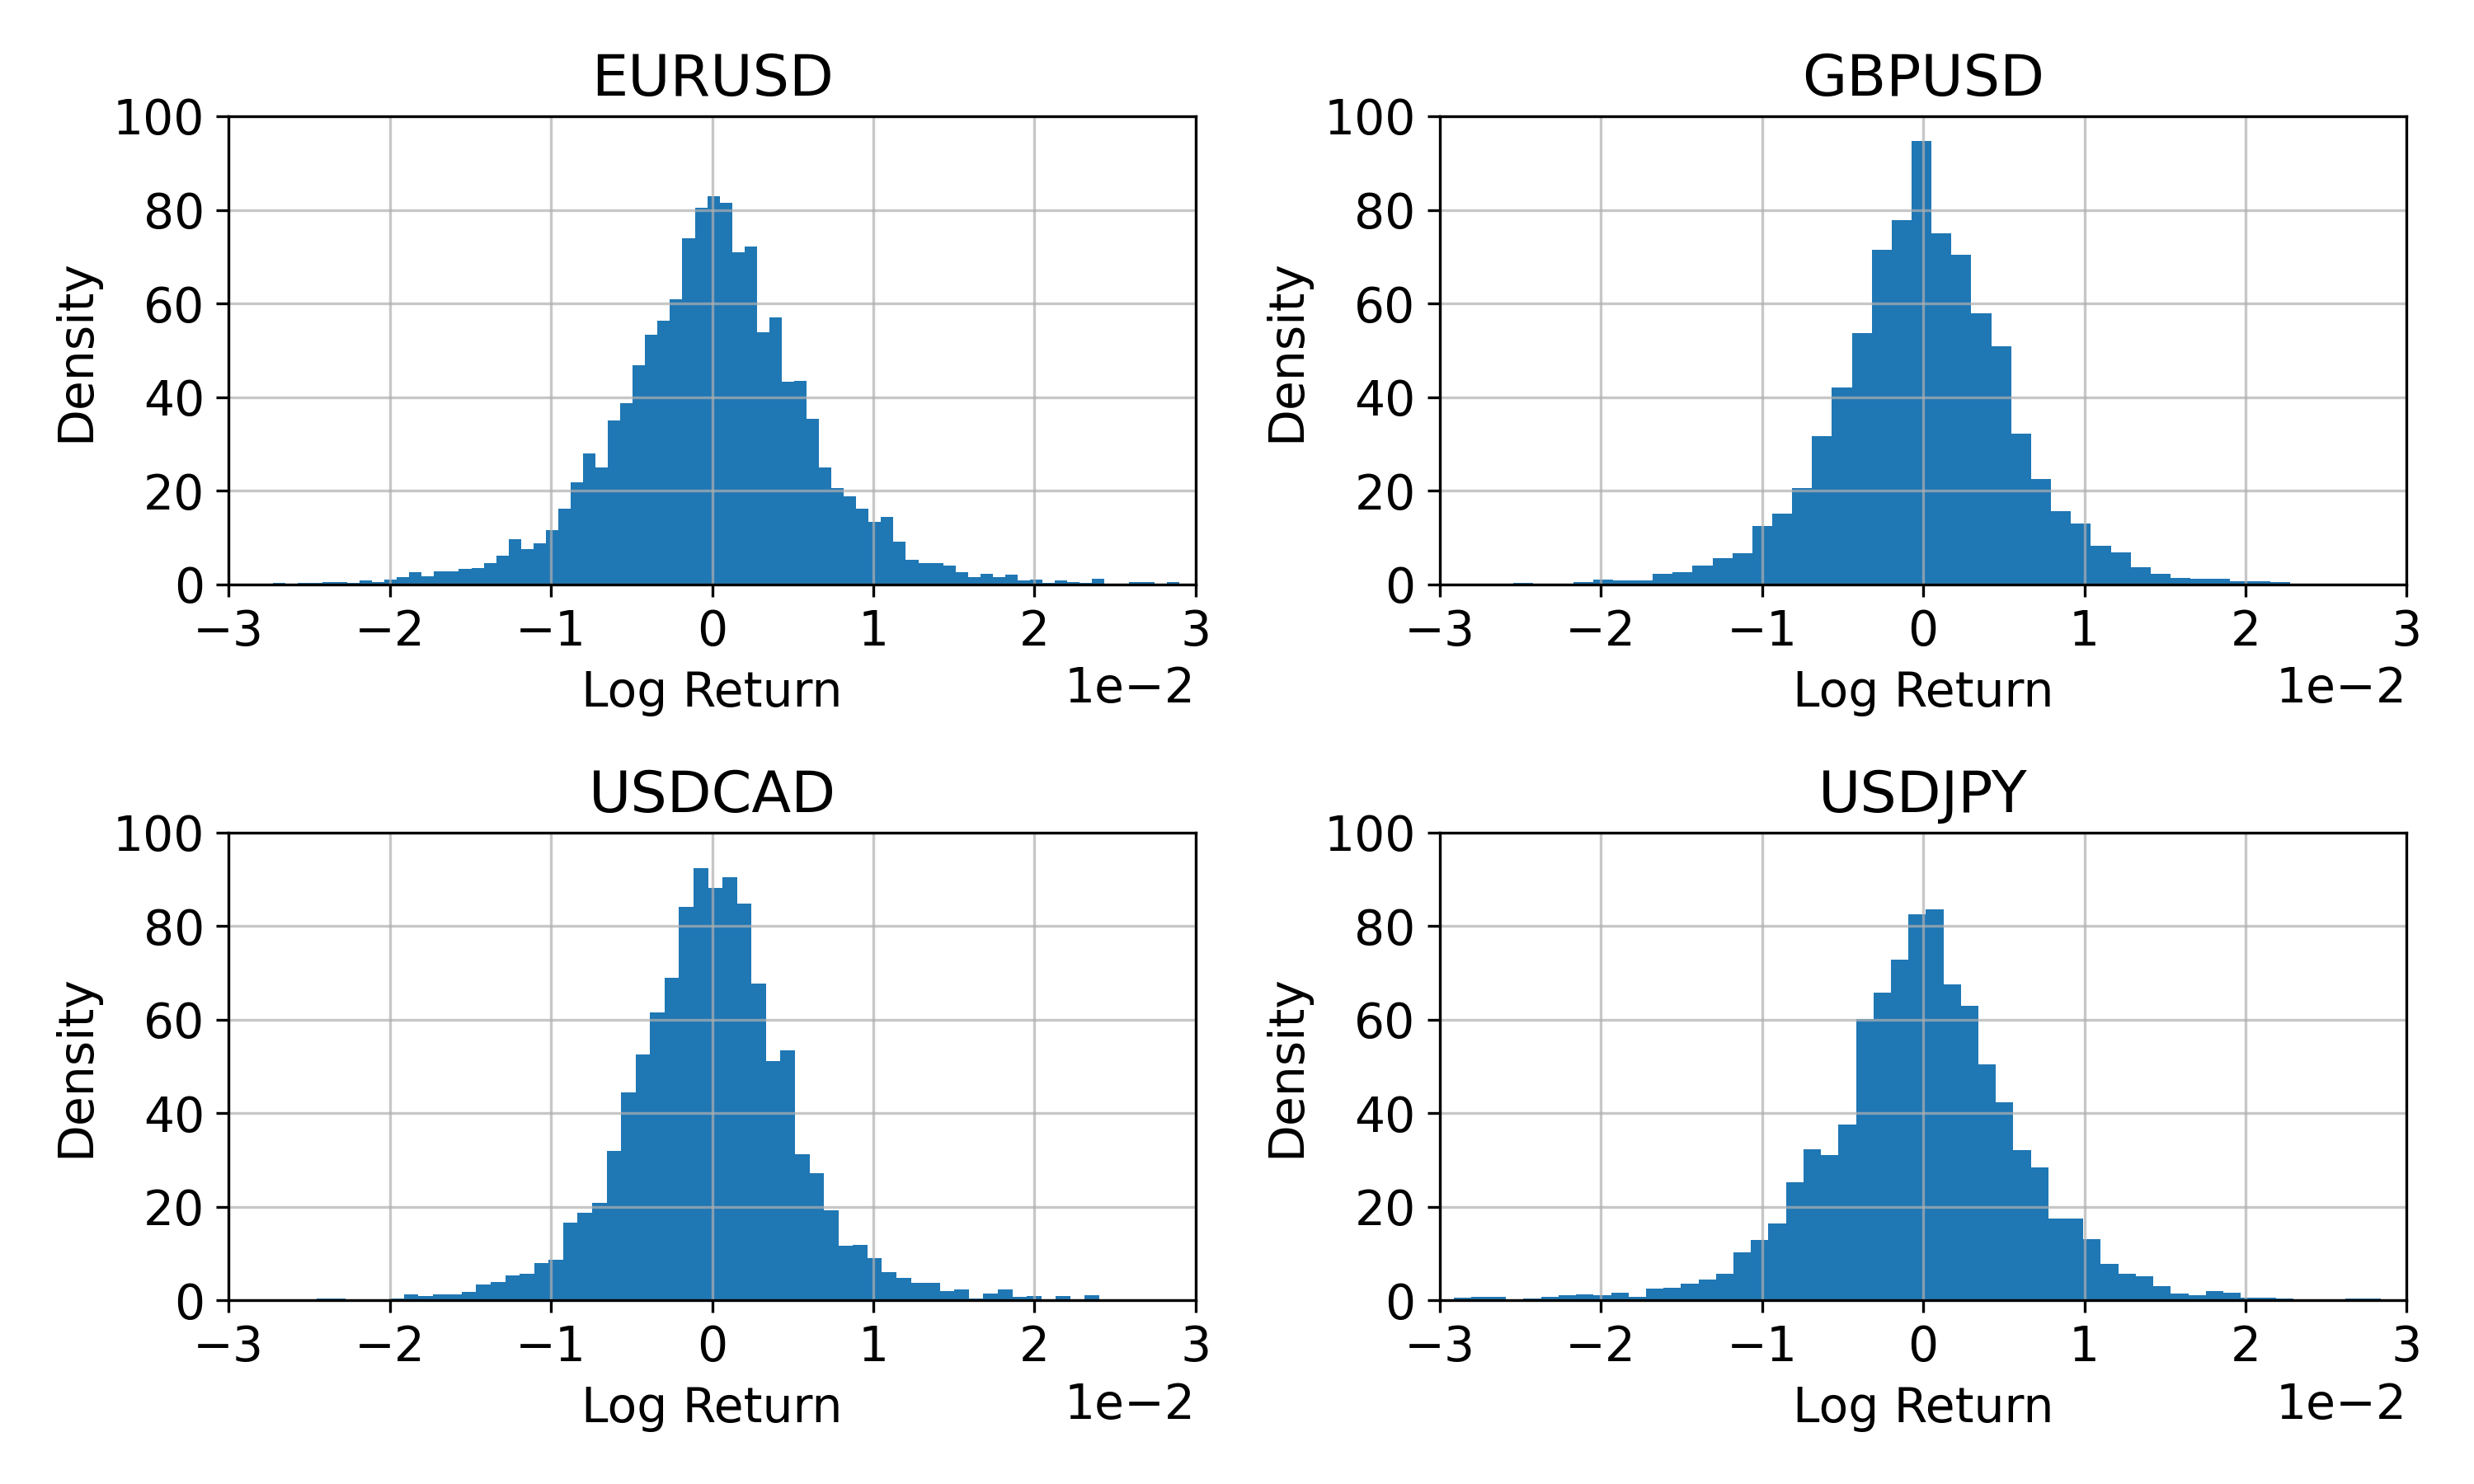
\includegraphics[width=1\linewidth]{data_analysis/histograms.png}
    \end{center}
    \caption{Histograms of the log returns data set.}
    \label{fig:histograms_raw}
\end{figure}

\begin{table}[!htb]
    \centering
    \begin{adjustbox}{max width=\textwidth}
        \input{../tables/data/log_returns_raw_stats.tbl}
    \end{adjustbox}
    \caption{Statistics of the log returns data set.}
    \label{tbl:data_log_returns_raw_stats}
\end{table}

We also visualize the log returns in a violin and box plot in~\cref{fig:violin_raw} to identify outliers and see how they are distributed.
Two major outliers clearly stand out from the rest: one to the downside for the GBPUSD pair, and the other to the upside for the USDJPY pair.
The former occurred on 2016-06-24, the day the Brexit referendum result was announced~\cite{brexit_gov_uk}.
The latter occurred on 2008-10-28, right in the midst of the financial crisis when people were talking about the end of the Yen carry trade~\cite{jpy_carry_trade_nyt}.
In the final training data set, we remove outliers greater than \( 10\sigma \) from the mean, resulting in only removing the day corresponding to the Brexit referendum result, which lies \( 11.1\sigma \) below the mean.
\begin{figure}[!htb]
    \begin{center}
        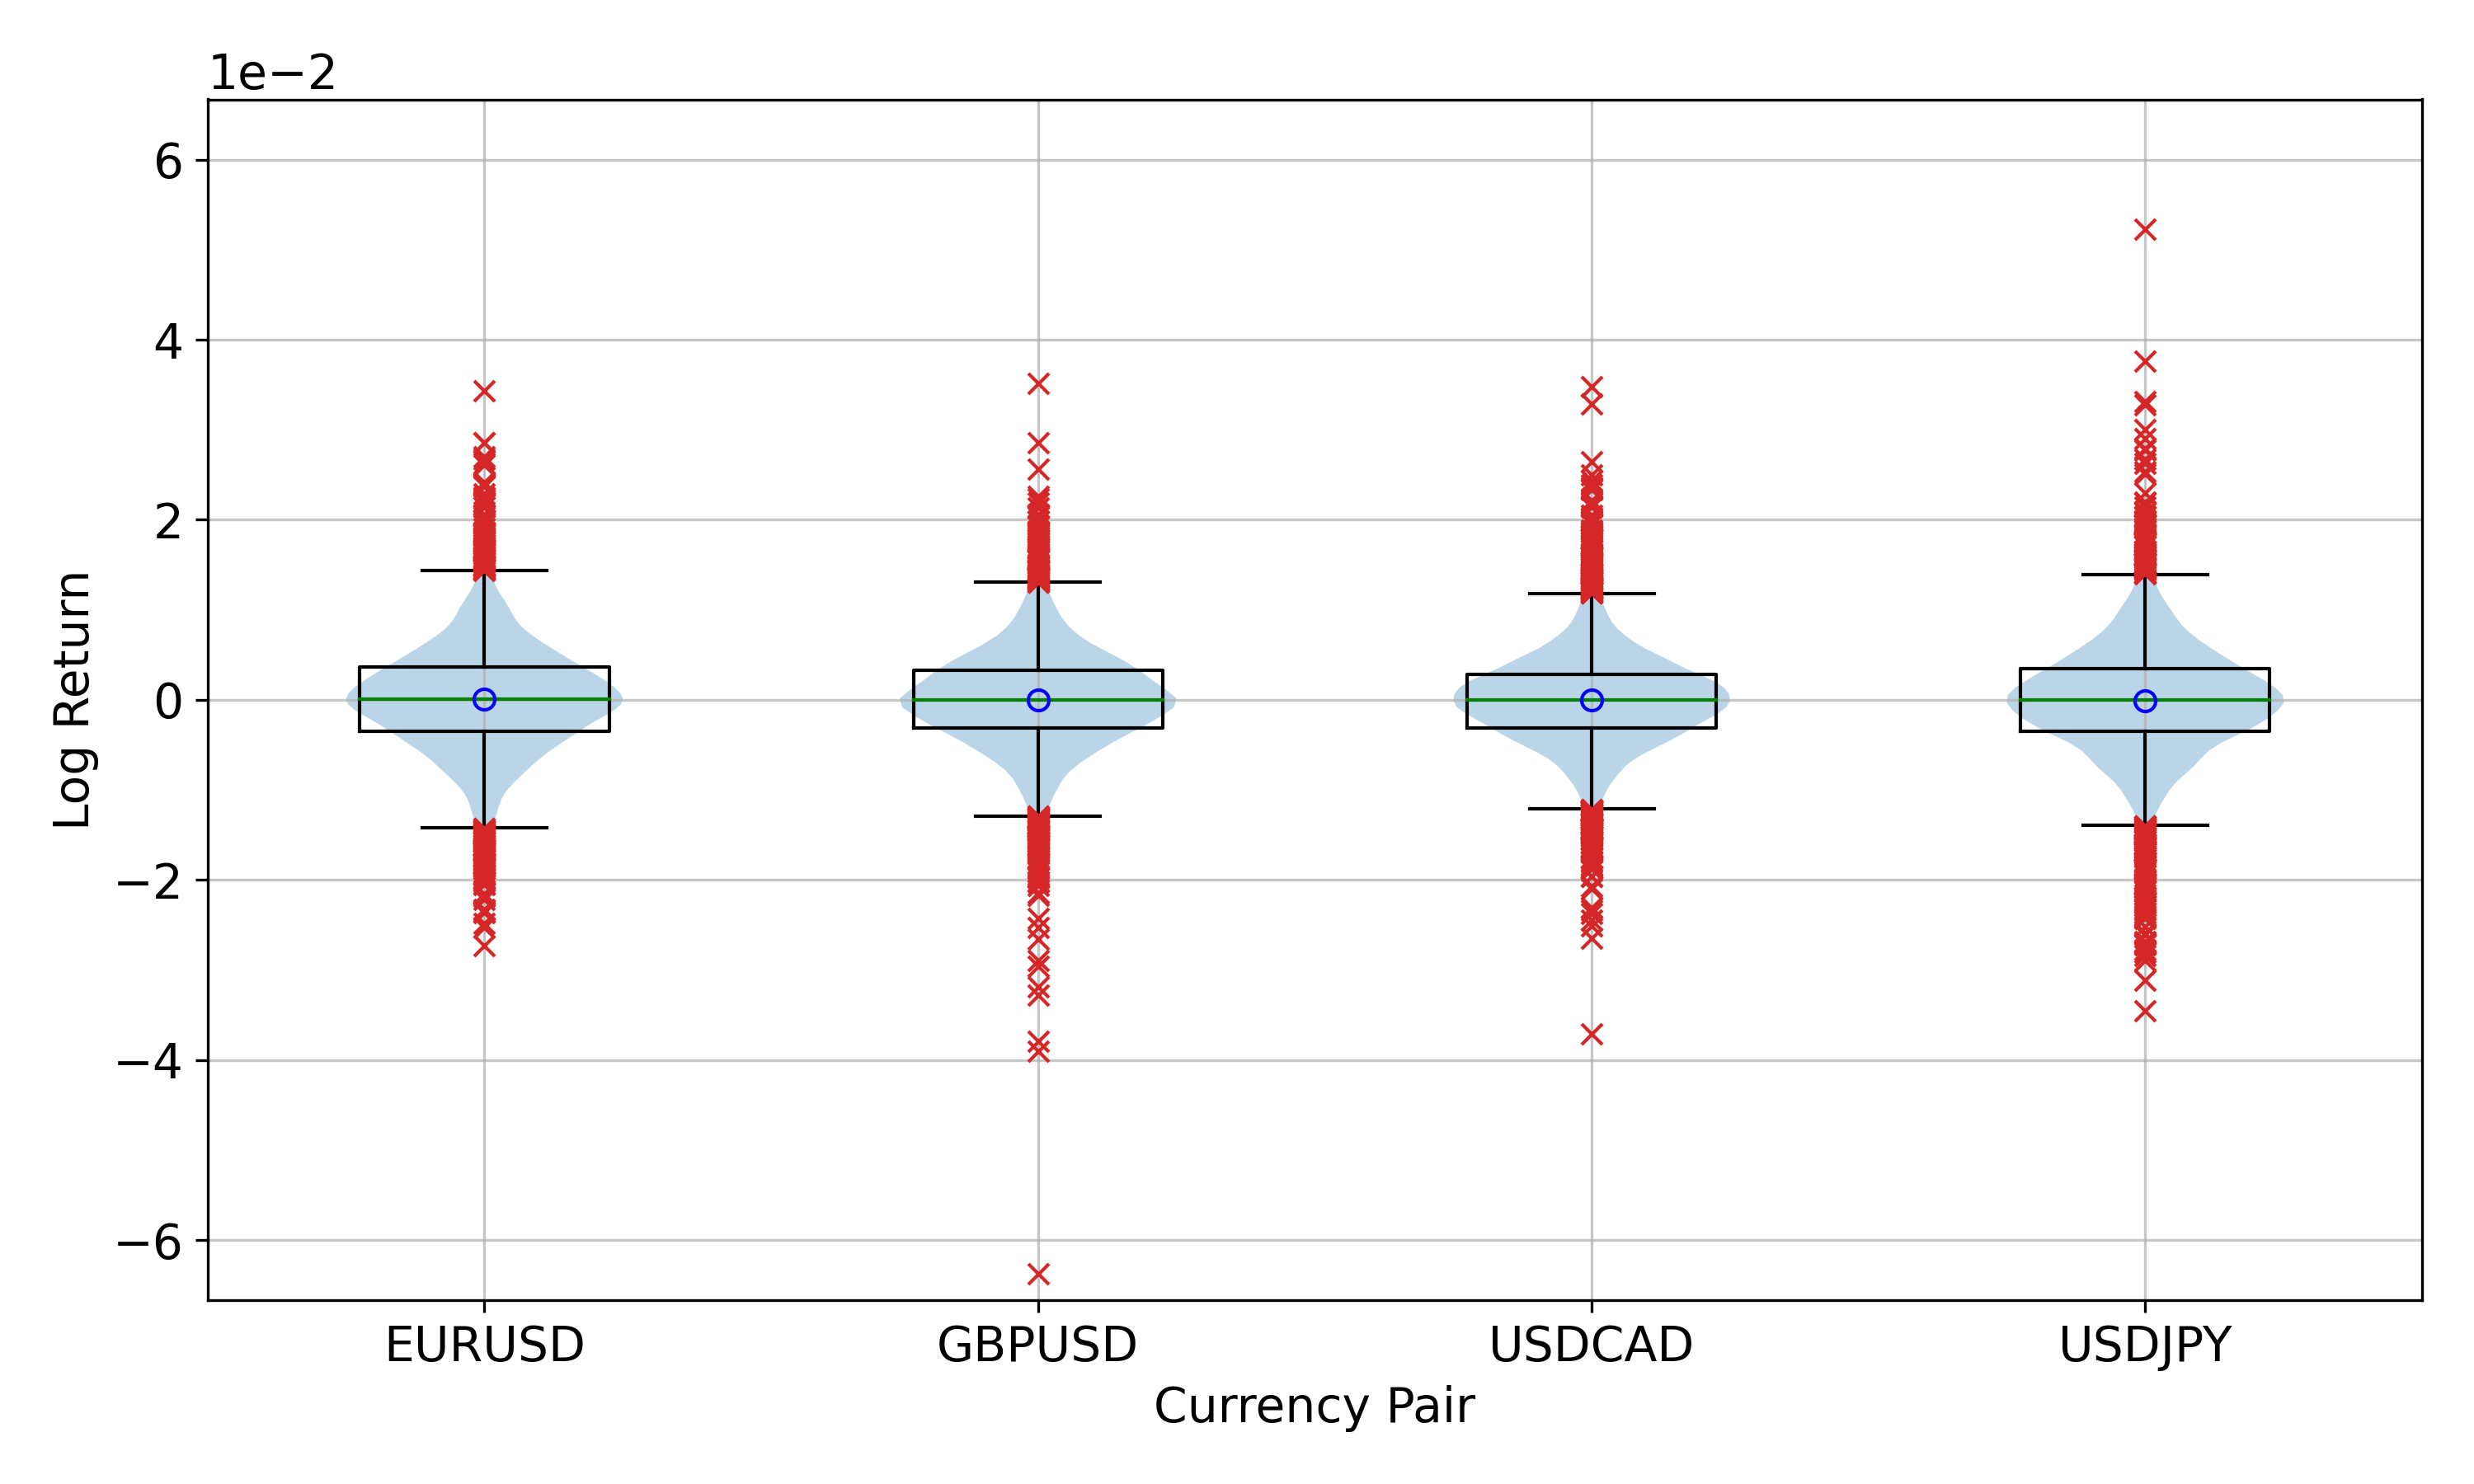
\includegraphics[width=1\linewidth]{data_analysis/violin.png}
    \end{center}
    \caption{Violin and box plot of the log returns data set illustrating the distribution of the outliers.}
    \label{fig:violin_raw}
\end{figure}

Next we examine the correlations between the currency pairs to get an idea of the interdependencies between them.
We visualize this with scatter plots shown in~\cref{fig:scatters} where we observe a clear positive correlation between EURUSD/GBPUSD, and clear negative correlations between EURUSD/USDCAD and GBPUSD/USDCAD, where the / is used to denote the pairs being compared against each other.
This is further verified by the Pearson \( r \), Spearman \( \rho \), and Kendall \( \tau \) correlation coefficients laid out in~\cref{tbl:data_correlation_coefficients}.
Furthermore, we find the correlation coefficients to be positive for pairs of the form \( X \)USD/\( Y \)USD, and negative for pairs of the form \( X \)USD/USD\( Y \), for \( X,Y \in \) \{EUR, GBP, CAD, JPY\}, as expected.
Details on how the correlation coefficients are computed and how to interpret them can be found in~\cref{app:correlation_coefficients}.
\begin{figure}[!htb]
    \begin{center}
        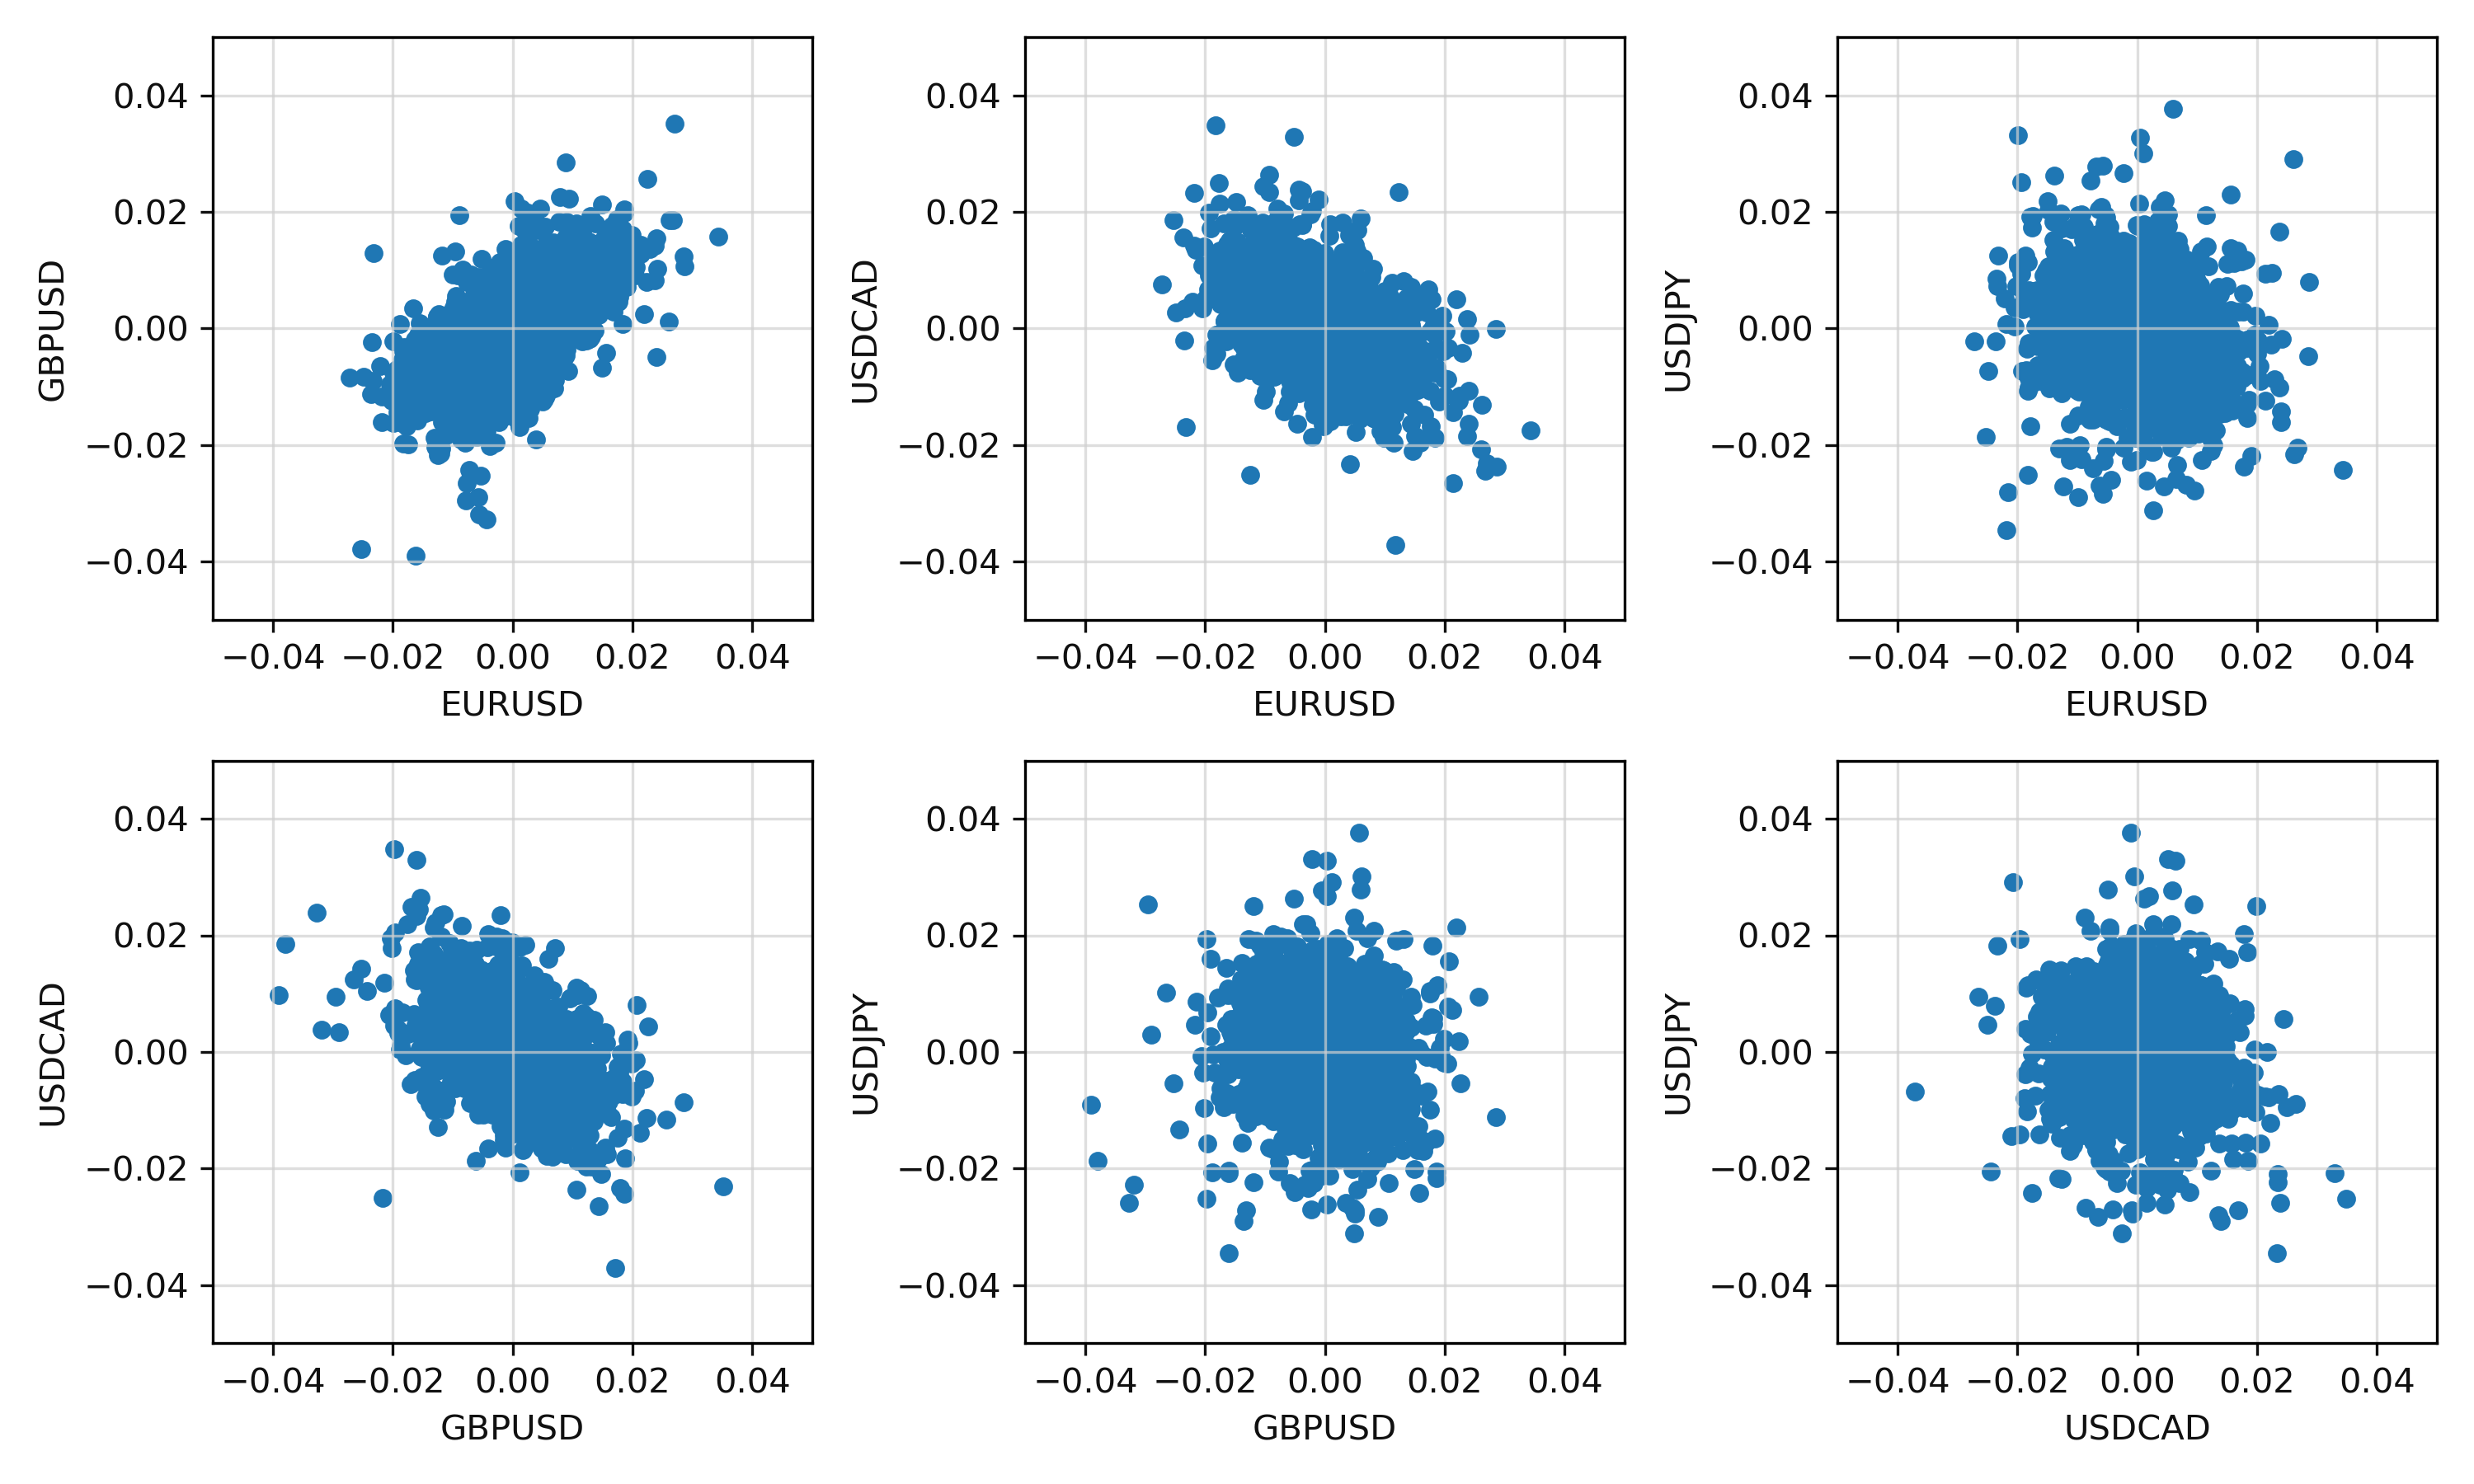
\includegraphics[width=1\linewidth]{data_analysis/scatters.png}
    \end{center}
    \caption{Scatter plots of the log returns data set.}
    \label{fig:scatters}
\end{figure}

\begin{table}[!htb]
    \centering
    \begin{adjustbox}{max width=\textwidth}
        \input{../tables/data/correlation_coefficients.tbl}
    \end{adjustbox}
    \caption{Correlation coefficients of the log returns data set.}
    \label{tbl:data_correlation_coefficients}
\end{table}


\section{Data Preprocessing}
The models in the following chapters require the training data to be in the form of bit vectors, so we must first convert our data set to such a form.
Let \( \mat{X} \in \R^{4 \times N} \) represent the training data set of log returns with \( N \) samples, where training samples are vectors in the column space, thus element \( x_{ij} \) represents the \( i \)th currency pair log return for the \( j \)th training sample.

To discretize the data, we rescale and round the entries of \( \mat{X} \) to integer values in \( \{0, 1, \dots, 2^{n_\text{bits}} - 1\} \), represented by the matrix \( \mat{X}' \in \N^{4 \times N} \) with entries
\begin{align}
    x_{ij}' = \bigg\lfloor \frac{x_{ij} - \min_k \{x_{ik}\}}{\max_k \{x_{ik}\} - \min_k \{x_{ik}\}} \cdot (2^{n_\text{bits}} - 1) \bigg\rceil,
\end{align}
where \( \lfloor \ \cdot \ \rceil \) denotes rounding to the nearest integer.

A new matrix \( \mat{V} \in \binset^{4\cdot n_\text{bits} \times N} \) is then created with the columns being the \( n_\text{bits} \)-length bit vectors corresponding to the binary representation of the entries of the columns of \( \mat{X}' \) concatenated together.
For example, if \( \vec{x}' = (x_1',x_2',x_3',x_4') \) is a column of \( \mat{X}' \) and the function \( \text{bitvector}(x') \) takes in an integer \( x' \) and returns an \( n_\text{bits} \)-bit binary representation bit vector, then the corresponding column in \( \mat{V} \) is
\begin{align}
    \vec{v} = \begin{bmatrix}
        \text{bitvector}(x_1') \\
        \text{bitvector}(x_2') \\
        \text{bitvector}(x_3') \\
        \text{bitvector}(x_4') \\
    \end{bmatrix}
    \in \binset^{4\cdot n_\text{bits}}.
\end{align}

For this research we take \( n_\text{bits} = 16 \), giving us a training set \( \mat{V} \in \binset^{64 \times N} \), thus our training samples are bit vectors of length 64.
The discretization errors associated with this conversion and data set are on the order of \( 10^{-7} \), well within the desired tolerance for this purpose.

\subsection{Data Transformation}\label{sec:outlier_transform}
Due to how the data is linearly converted to a discrete form before rounding, it opens up the possibility of the discretized data being clustered in the mid-range values if large outliers are present.
To mitigate this, we use a transformation to reduce the gap between outliers by scaling outliers beyond a certain threshold \( \tau \) using the procedure detailed in~\cref{alg:transformation}.
We call this the \textit{outlier power transformation}.
In practice, we take \( \tau = 1 \) and \( \alpha = 0.5 \), thus the standardized data points above one standard deviation are mapped to their square roots, as illustrated in~\cref{fig:data_transformation}.
We tested a few other combinations of \( \tau \) and \( \alpha \), but found these values to produce the best model results out of those we tried; of course this could likely be further optimized.
This transformation is invertible when \( \bar{x} \), \( \sigma_x \), and \( \delta \) are saved.

\begin{algorithm}
\caption{Outlier Power Transformation}
\begin{algorithmic}[1]
    \Procedure{Transform}{$\vec{x}, \alpha, \tau$}
            \Comment $\alpha$ is the power, $\tau$ is the threshold
        \State $N \gets \text{length}(\vec{x})$
        \State $\bar{x} \gets \frac{1}{N} \sum_{i=1}^{N} x_i$
        \State $\sigma_{x} \gets \sqrt{\frac{1}{N} \sum_{i=1}^{N} (x_i - \bar{x})^2}$
        \State $\delta \gets \tau - \tau^\alpha$
            \Comment ensures the transformation is bijective
        \For {$i$ in 1 to $N$}
            \State $x_i \gets (x_i - \bar{x}) / \sigma_x$
                \Comment standardize
            \If {$x_i > \tau$}
                \State $x_i \gets (\abs{x_i}^\alpha + \delta) \cdot \text{sign}(x_i)$
                    \Comment scale standardized values beyond $\tau$
            \EndIf
            \State $x_i \gets x_i \cdot \sigma_x + \bar{x}$
                \Comment undo standardization
        \EndFor
    \EndProcedure
\end{algorithmic}
\label{alg:transformation}
\end{algorithm}

\begin{figure}[!htb]
    \begin{center}
        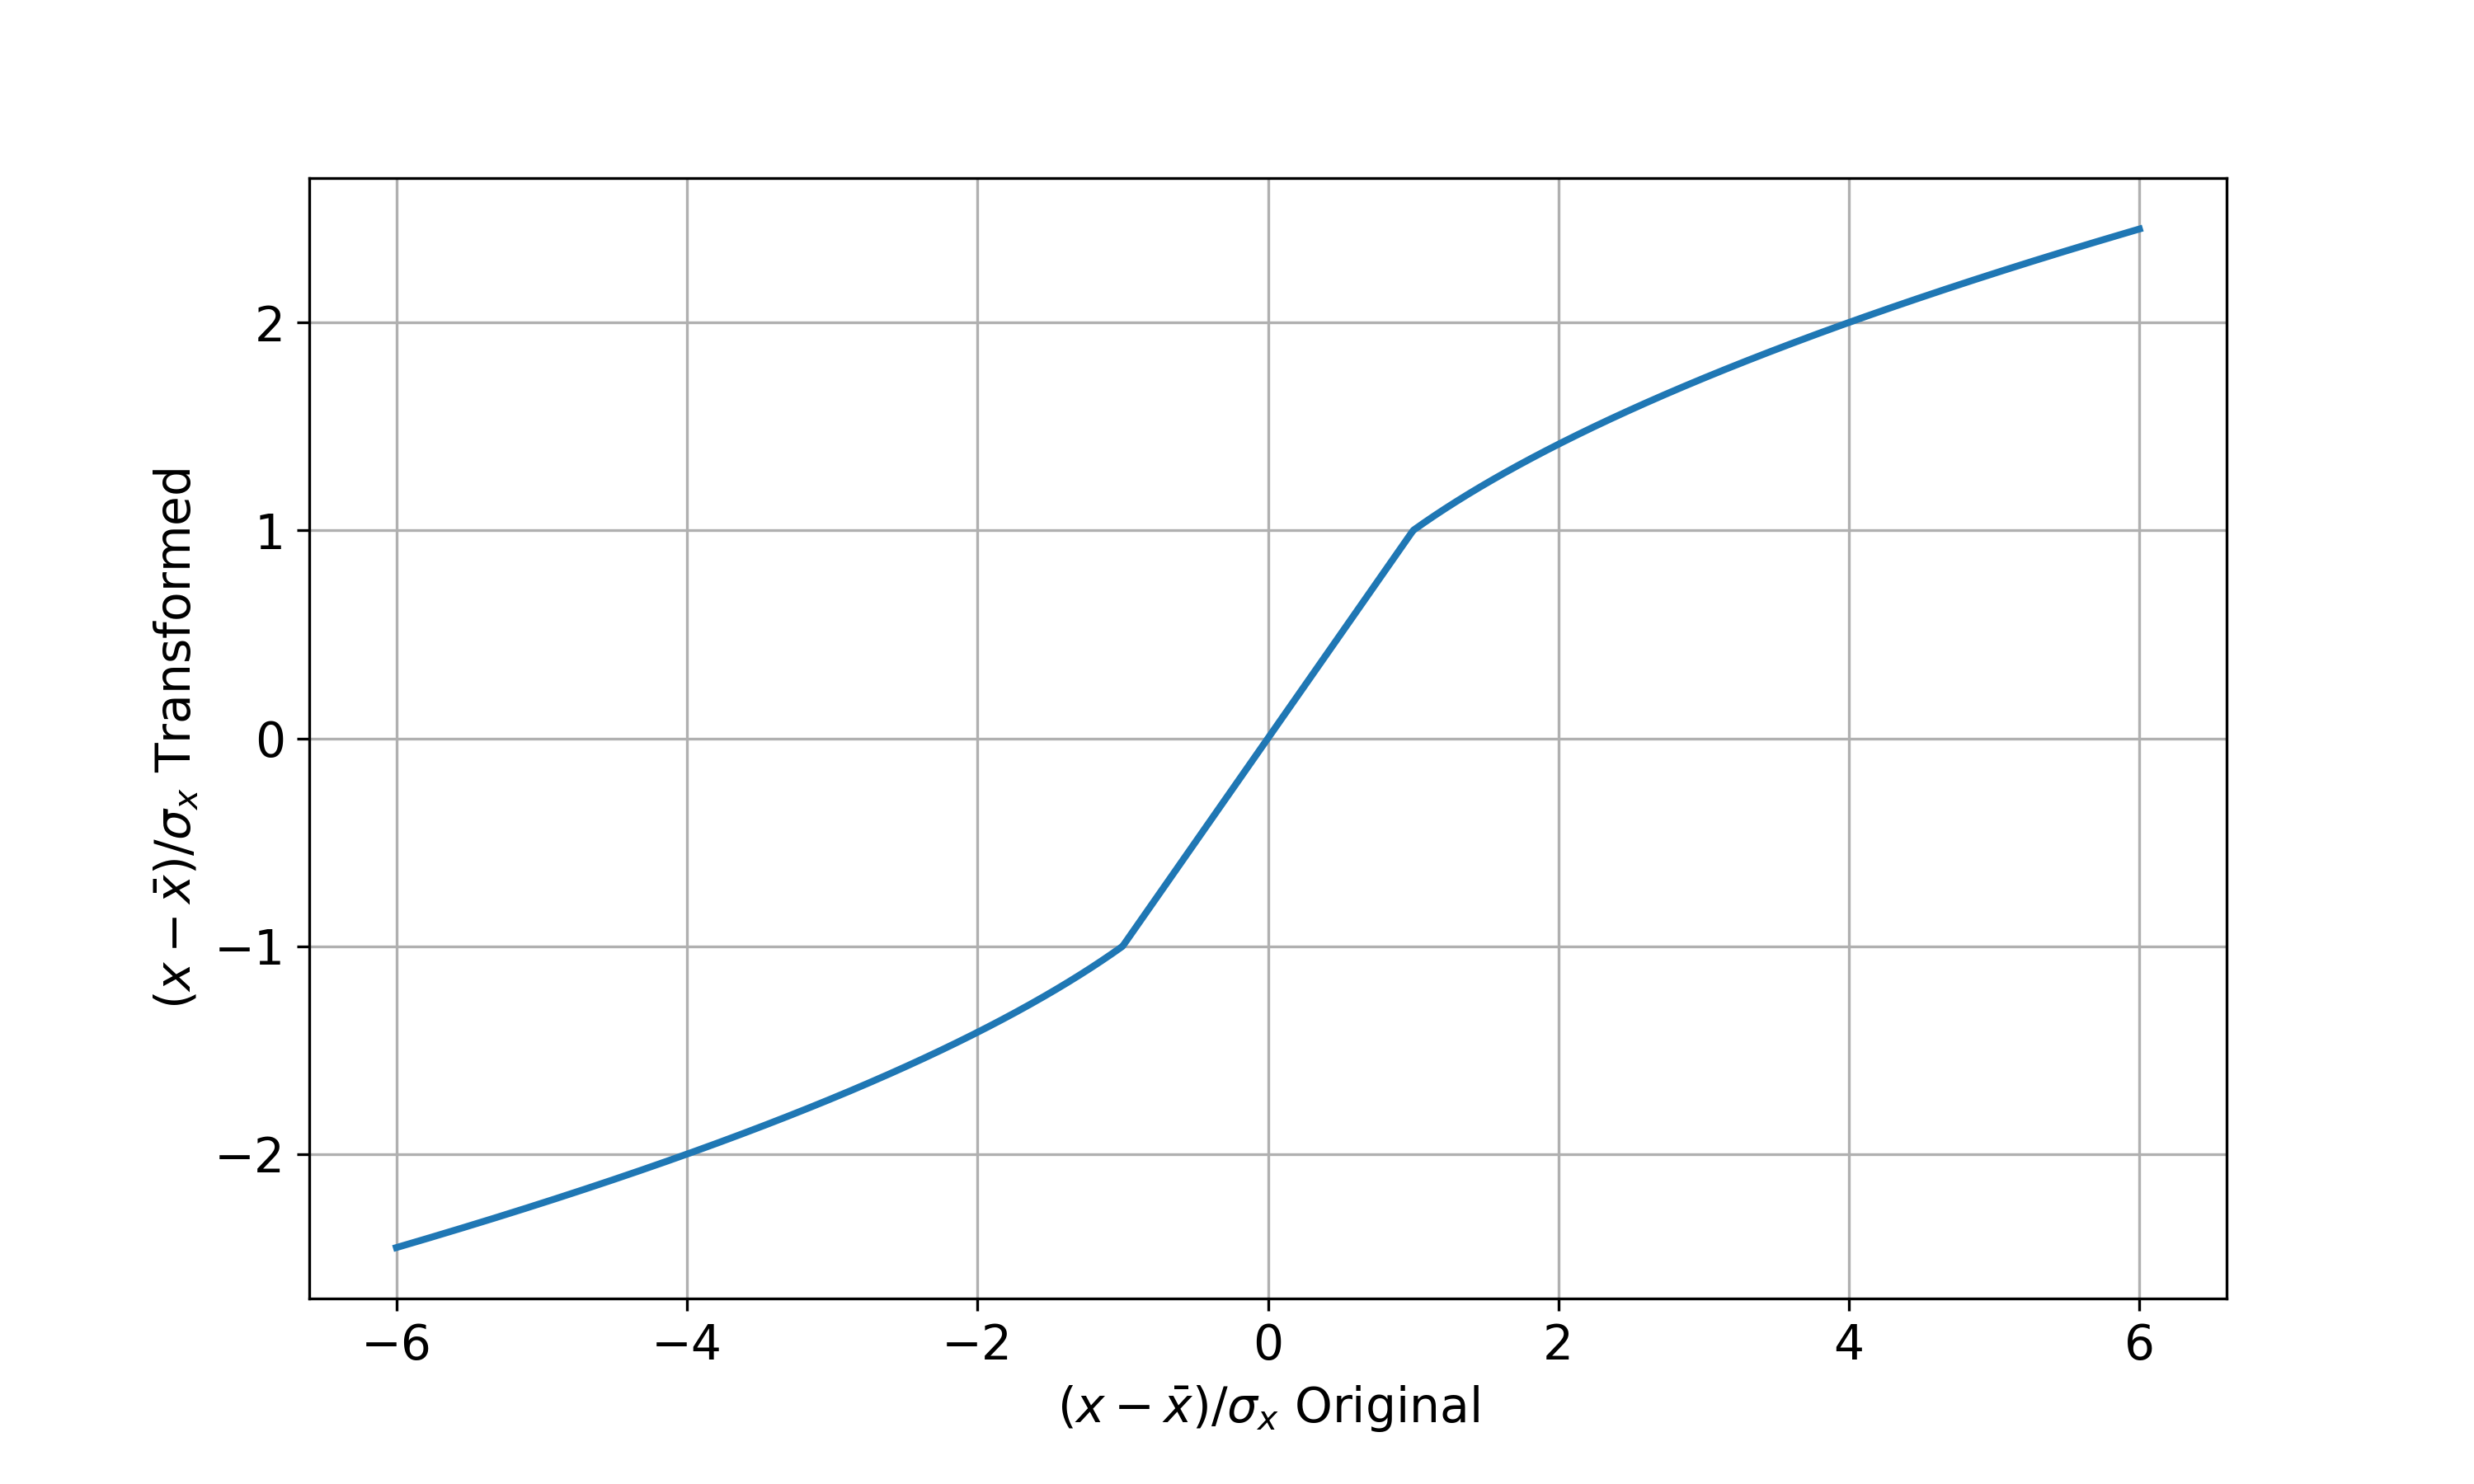
\includegraphics[width=1\linewidth]{data_analysis/data_transformation.png}
    \end{center}
    \caption{Transformation defined in~\cref{alg:transformation} using \( \tau = 1 \) and \( \alpha = 0.5 \), for the purpose of reducing large gaps in the discretized data set by scaling outliers above \( \tau \) standard deviations.}
    \label{fig:data_transformation}
\end{figure}

Histograms of the transformed data set are shown in~\cref{fig:histograms_transformed}, and a violin and box plot is shown in~\cref{fig:violin_transformed}.
In these, we observe the appearance of "shoulders" around the threshold \( \tau = 1 \) standard deviation, and that the transformed outliers appear much less extreme, allowing us to better utilize the full range of discrete values.
\cref{tbl:data_log_returns_transformed_stats} shows that the transformation reduces the standard deviations to roughly \( 78\% \) of their originals values given in~\cref{tbl:data_log_returns_raw_stats}.

\begin{figure}[!htb]
    \begin{center}
        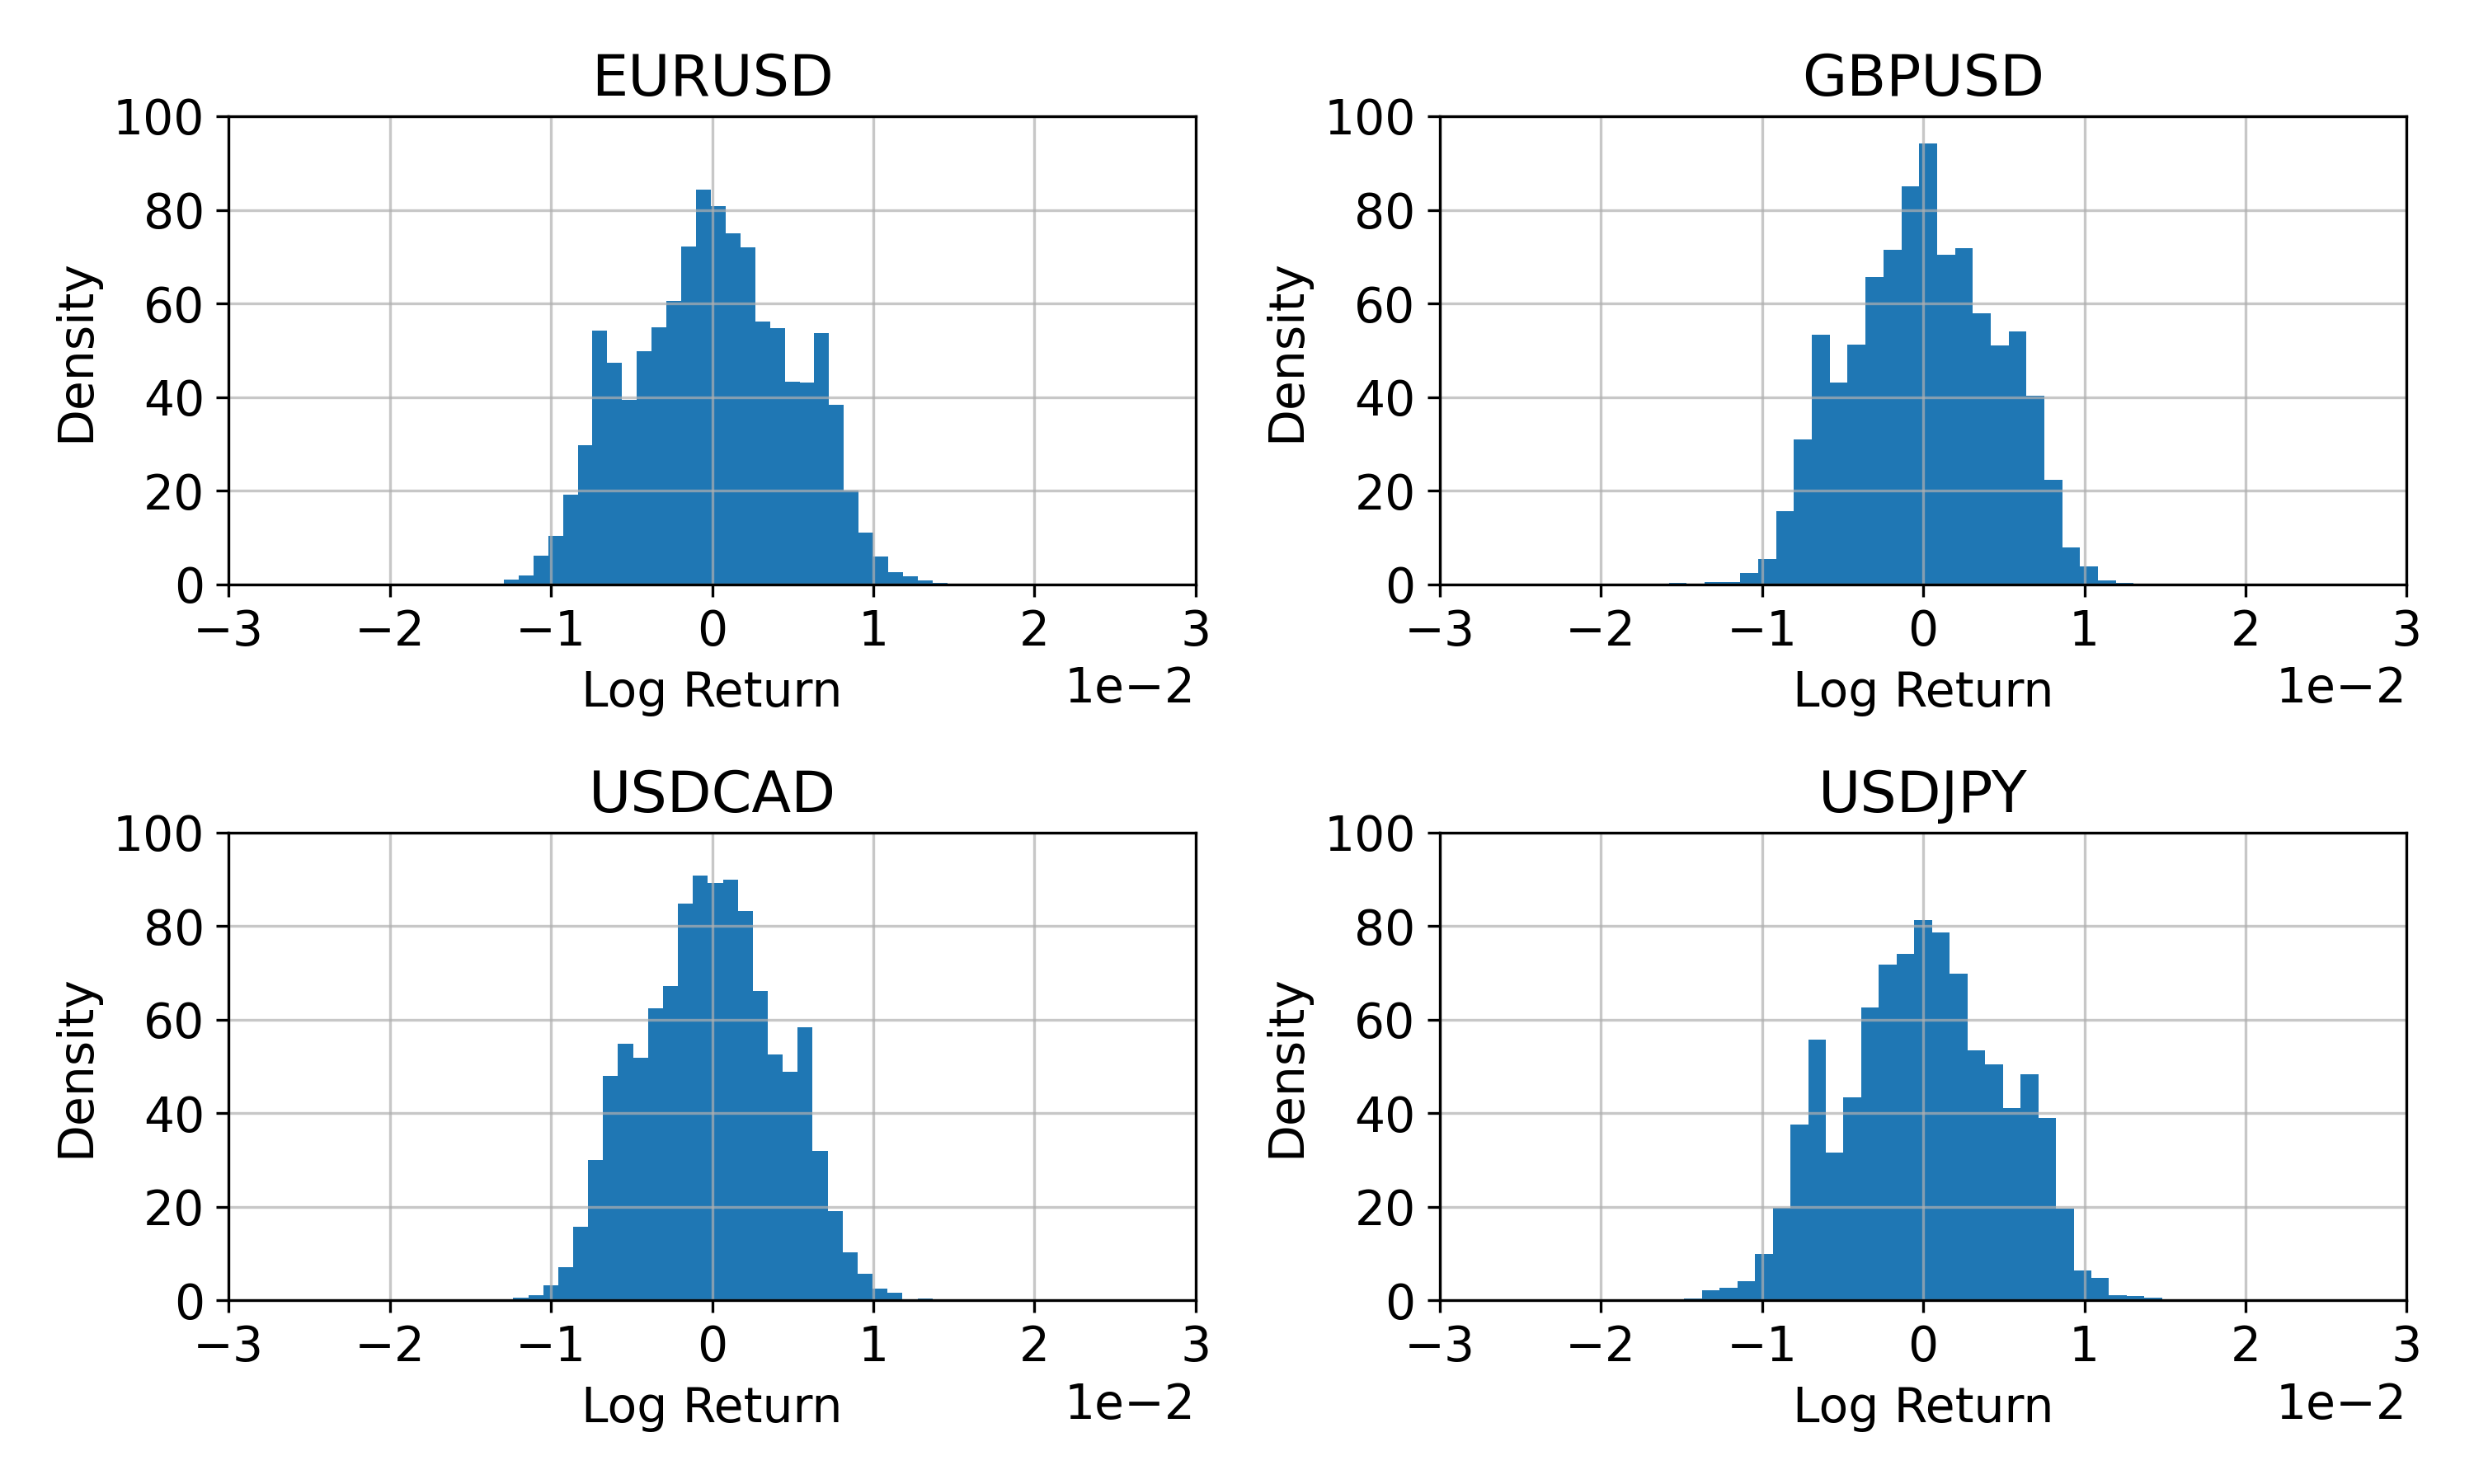
\includegraphics[width=1\linewidth]{data_analysis/histograms_transformed.png}
    \end{center}
    \caption{Histograms of the outlier power-transformed log returns data set.}
    \label{fig:histograms_transformed}
\end{figure}
\begin{figure}[!htb]
    \begin{center}
        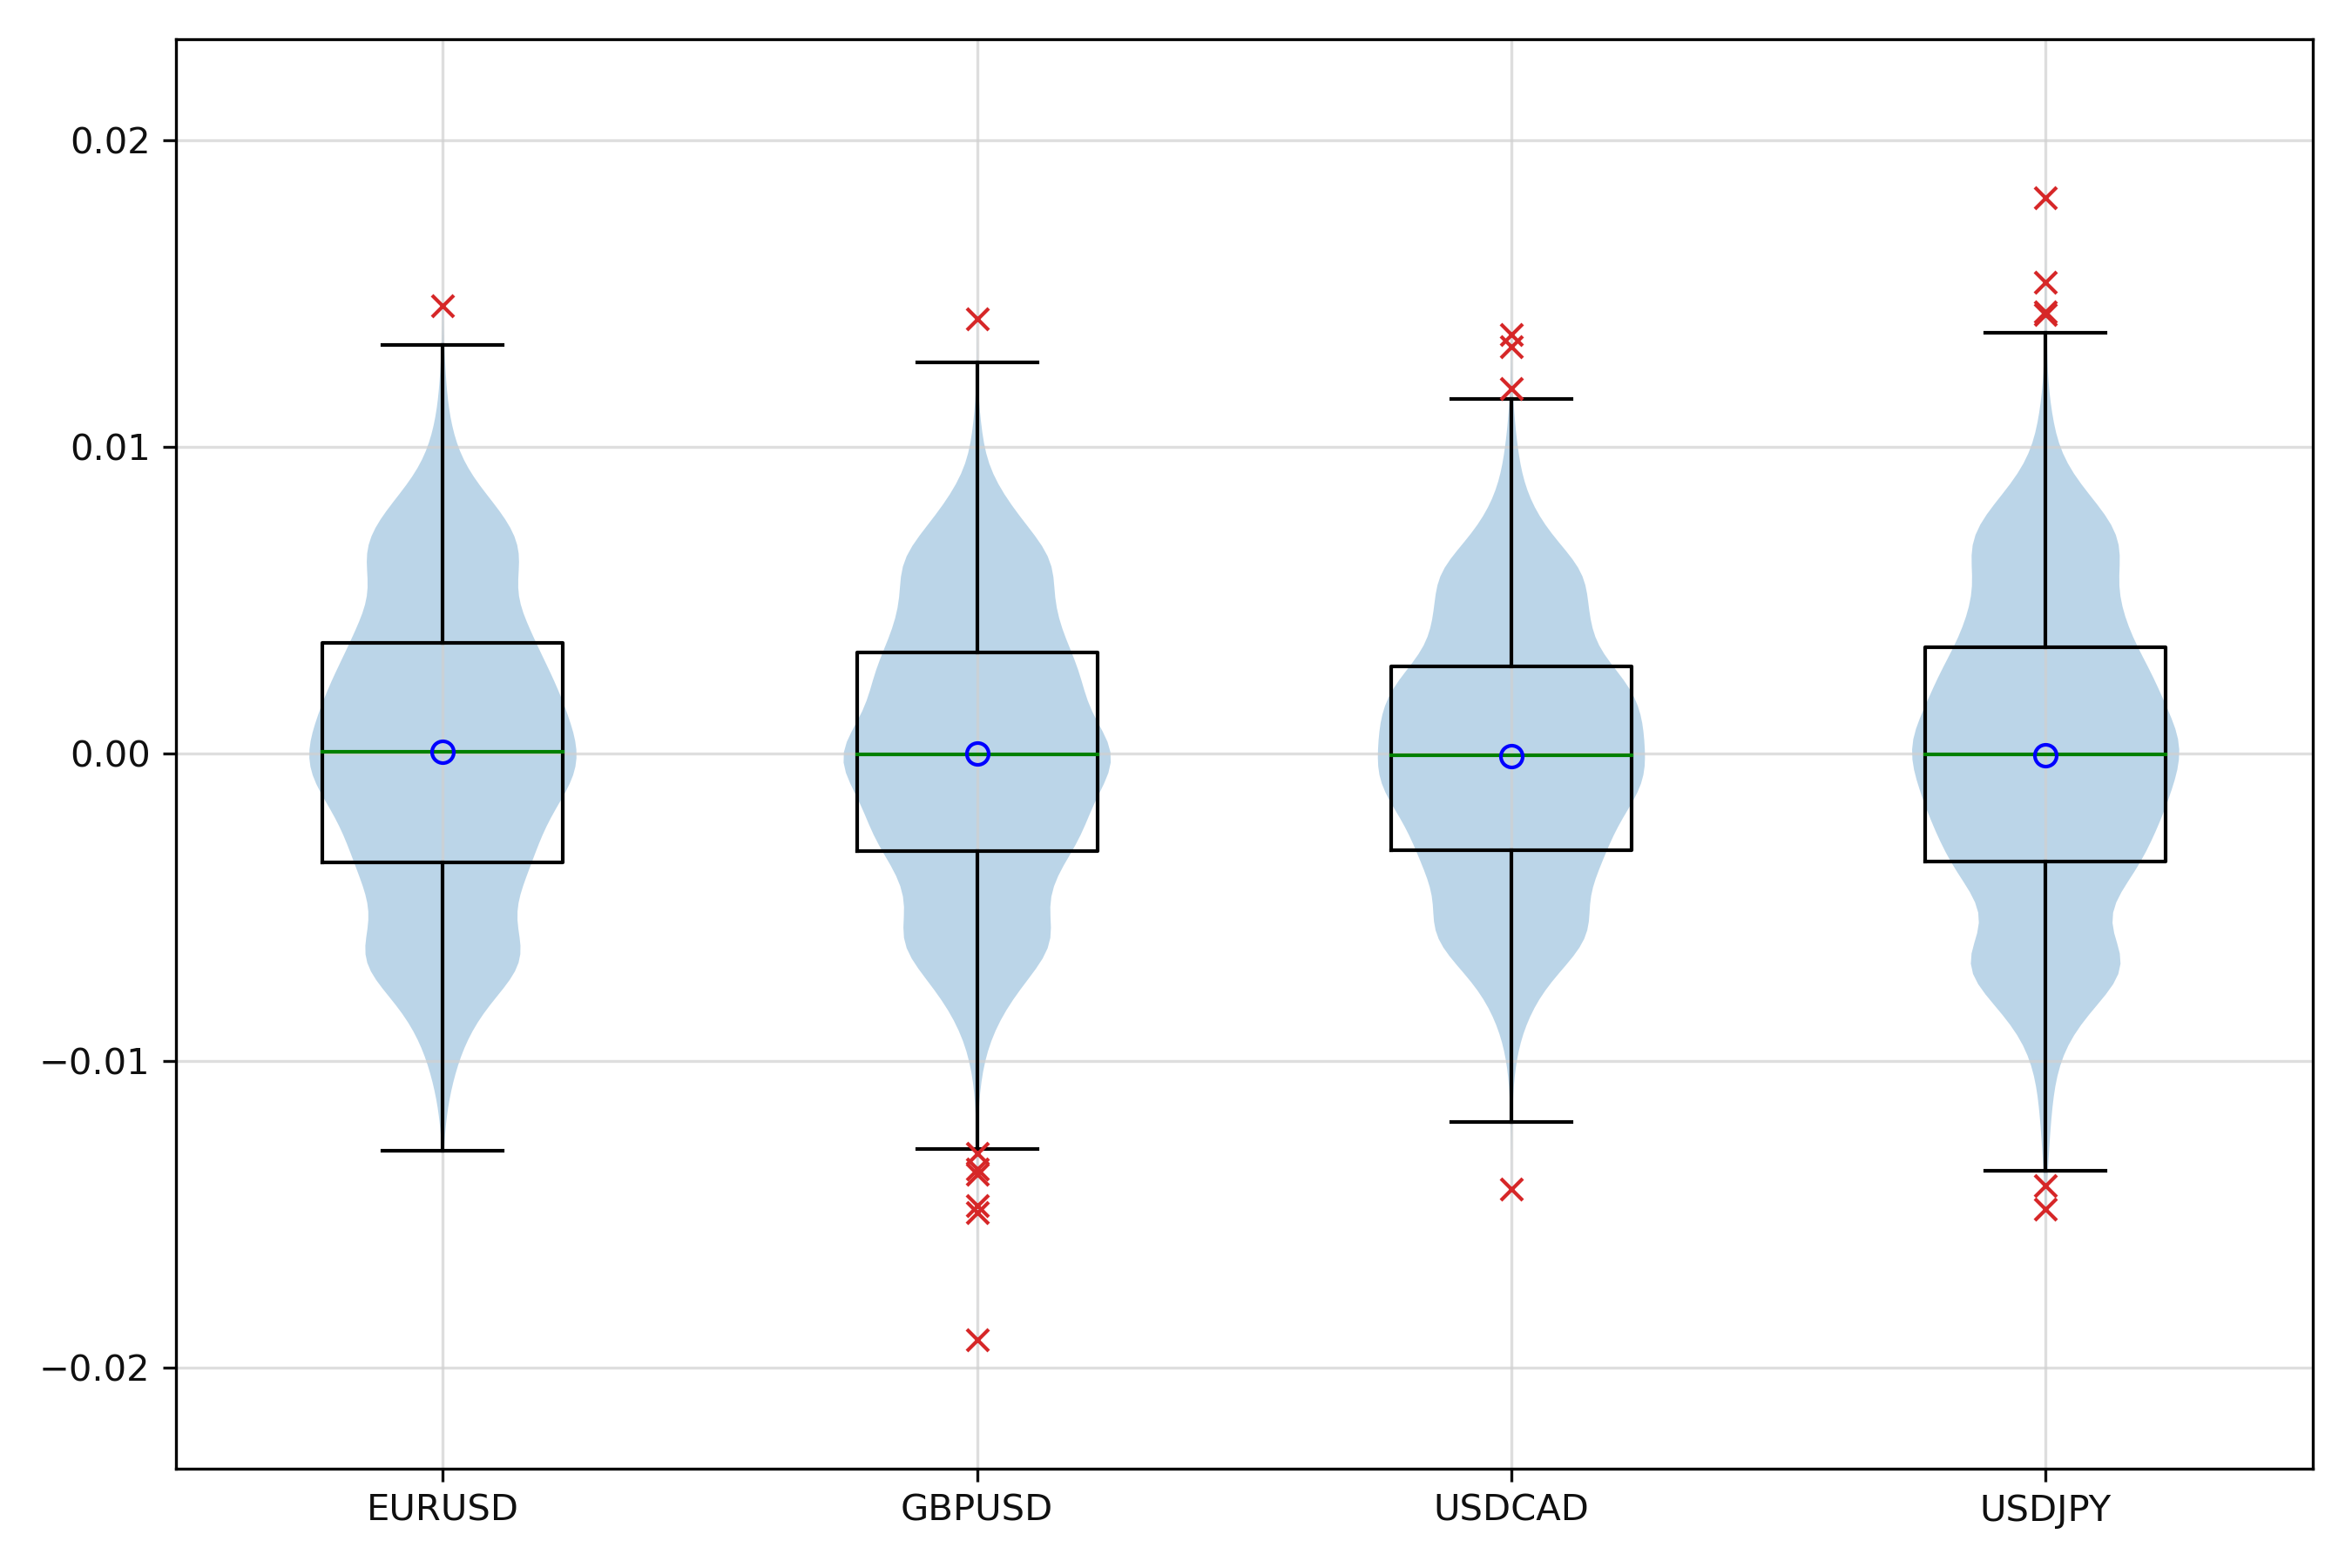
\includegraphics[width=1\linewidth]{data_analysis/violin_transformed.png}
    \end{center}
    \caption{Violin and box plot of the outlier power-transformed log returns data set illustrating the distribution of the rescaled outliers.}
    \label{fig:violin_transformed}
\end{figure}
\begin{table}[!htb]
    \centering
    \begin{adjustbox}{max width=\textwidth}
        \input{../tables/data/log_returns_transformed_stats.tbl}
    \end{adjustbox}
    \caption{Statistics of the outlier power-transformed log returns data set.}
    \label{tbl:data_log_returns_transformed_stats}
\end{table}

\subsection{Additional Information}
As mentioned in~\cite{kondratyev_2019}, one can use additional binary indicator variables to enrich the training data set.
One such bit of information is the rolling volatility relative to the historical median (see~\cref{app:annualized_volatility} for definition of annualized volatility).
If the 3-month rolling volatility is below (above) the historical median it is assigned a value of 0 (1) to indicate the low (high) volatility regime.
The 3-month rolling volatilities versus their historical medians are plotted in in~\cref{fig:rolling_volatility}.

These additional binary indicator variables are then concatenated onto the training data set and fed to the model to make it more flexible by allowing for the model outputs to be conditioned on a specific volatility regime.
Adding one indicator for each of the four currency pairs increases the number of rows in our training data set by four, thus the volatility-concatenated data set is in the space \( \binset^{68 \times N} \).

\begin{figure}[!htb]
    \begin{center}
        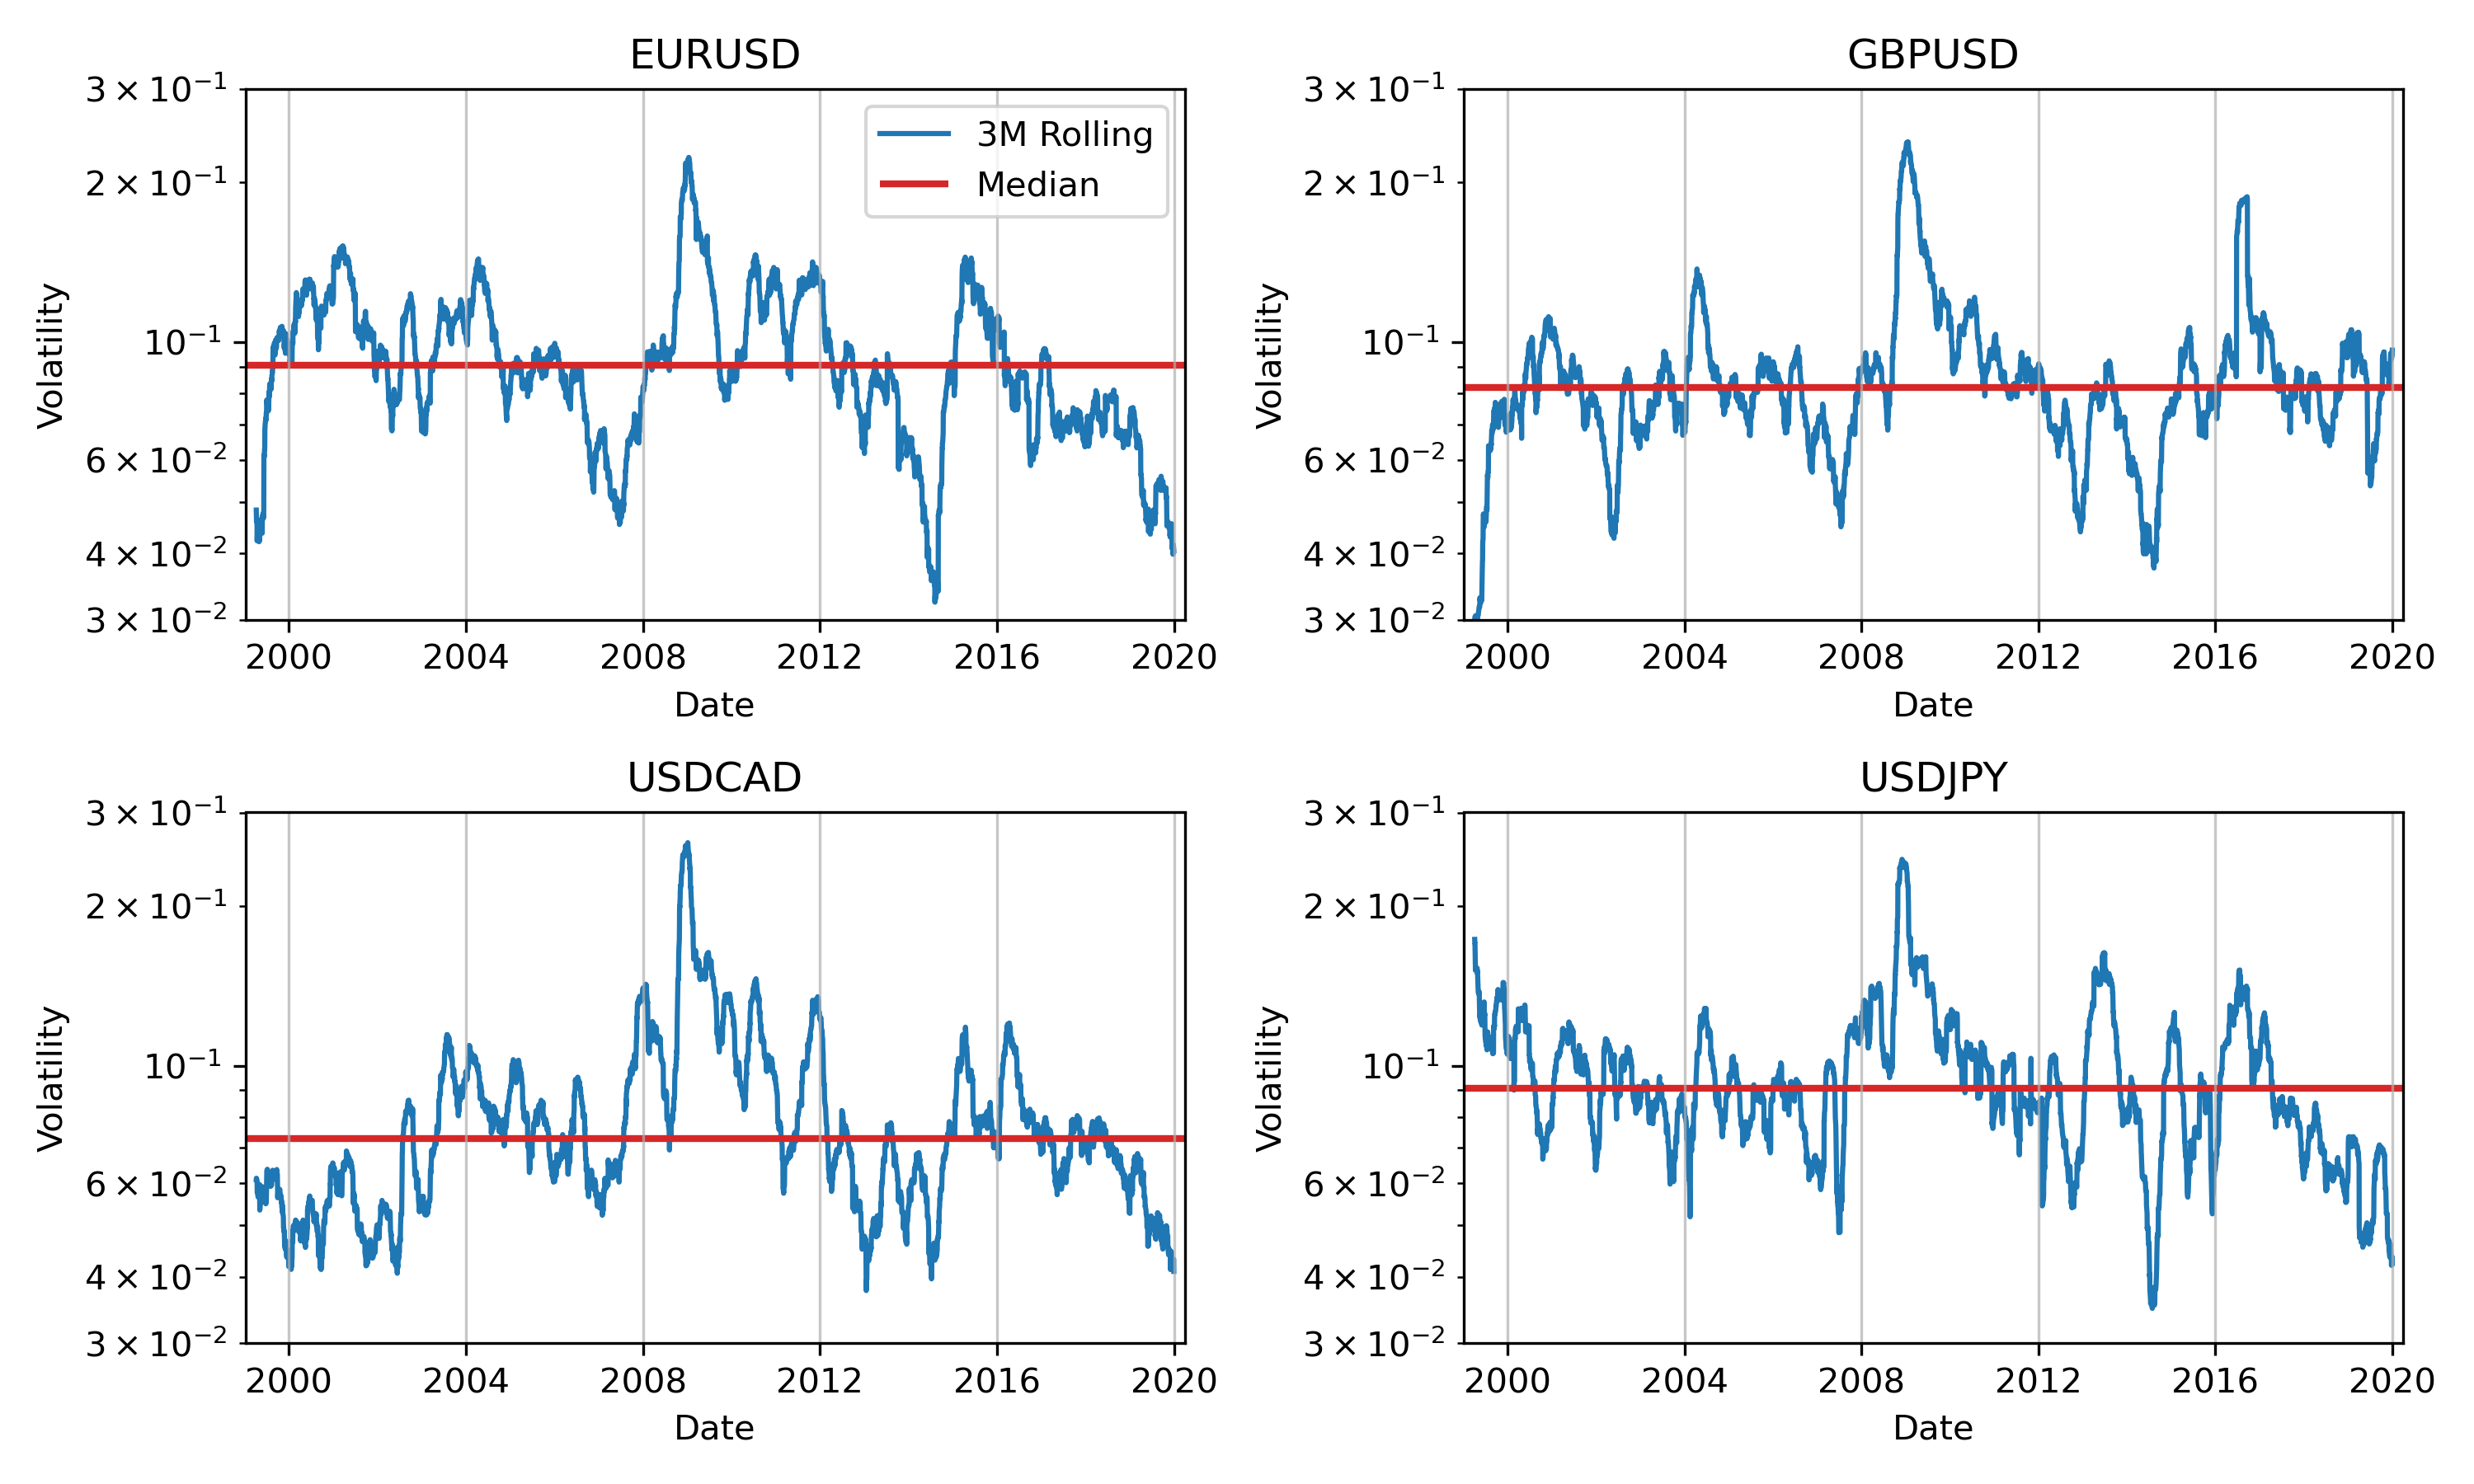
\includegraphics[width=1\linewidth]{data_analysis/rolling_volatility.png}
    \end{center}
    \caption{3-month rolling volatilities of the log returns data set compared with their historical medians.}
    \label{fig:rolling_volatility}
\end{figure}


%----------------------------------------------------------------------------------------
% RBM
%----------------------------------------------------------------------------------------
\chapter{Restricted Boltzmann Machine}
\label{ch:rbm}
\section{Theory}
\todo{Algorithm for Gibbs sampling}

\todo{Algorithm for contrastive divergence}

\todo{Derivation of log likelihood gradient (appendix)}

\begin{figure}
    \begin{center}
        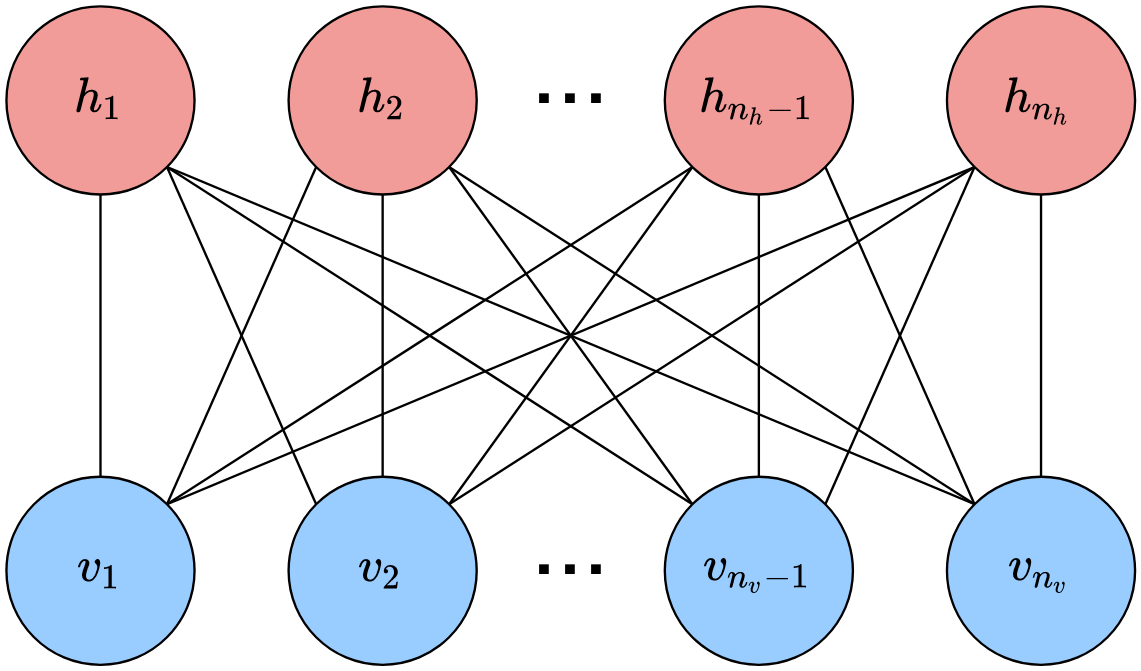
\includegraphics[width=1\linewidth]{rbm_diagram.png}
    \end{center}
    \caption{The structure of a restricted Boltzmann machine with \( n_v \) visible units and \( n_h \) hidden units.}
    \label{fig:rbm_diagram}
\end{figure}

\begin{figure}
    \begin{center}
        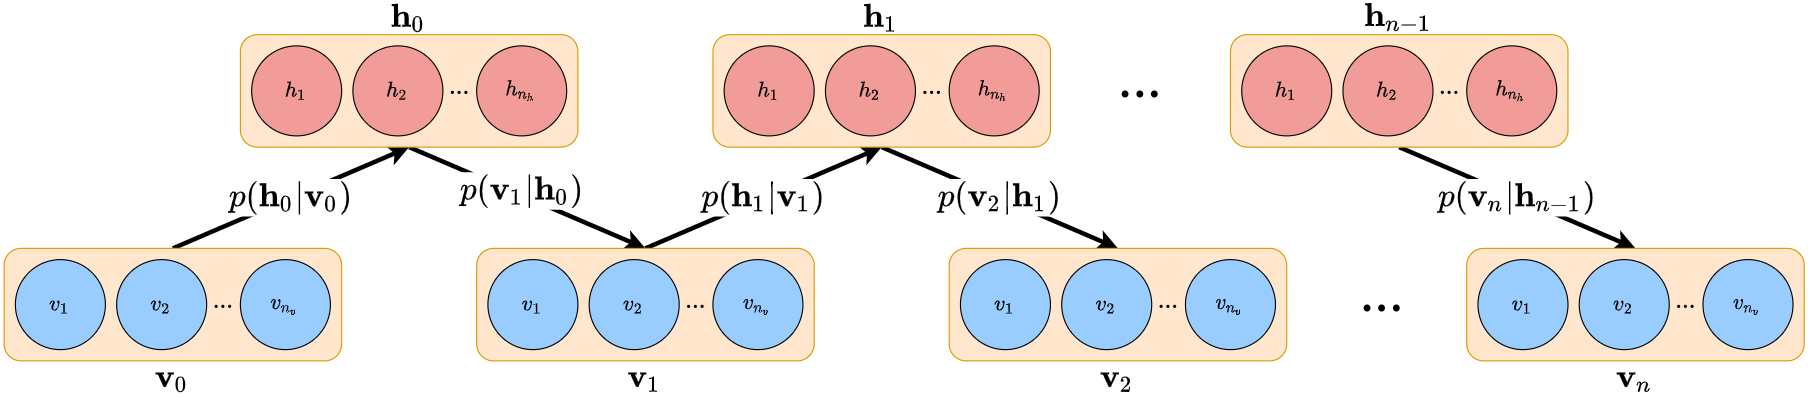
\includegraphics[width=1\linewidth]{gibbs_sampling_diagram.png}
    \end{center}
    \caption{Illustration of the Gibbs sampling procedure.}
    \label{fig:gibbs_sampling_diagram}
\end{figure}

\section{Application}

\section{Results}
In this section we will compare four different RBM models, denoted as:
\begin{itemize}
    \item (B): baseline model.
    \item (V): using volatility indicators.
    \item (X): using a transformed feature space.
    \item (XV): using a transformed feature space and volatility indicators.
\end{itemize}

\begin{table}[ht]
    \centering
    \begin{adjustbox}{max width=\textwidth}
        \input{../tables/rbm/correlation_coefficients.tbl}
    \end{adjustbox}
    \caption{Correlation coefficients of the data vs. samples generated by the RBM models. The RBM numbers are shown in the format average \(\pm\) 1 standard deviation from an ensemble of size 100.}
    \label{tbl:rbm_correlation_coefficients}
\end{table}

\begin{table}[ht]
    \centering
    \begin{adjustbox}{max width=\textwidth}
        \input{../tables/rbm/qq_rmses.tbl}
    \end{adjustbox}
    \caption{QQ root mean squared errors of the RBM models. All numbers are shown in the format average \(\pm\) 1 standard deviation from an ensemble of size 100.}
    \label{tbl:rbm_qq_rmse}
\end{table}

\begin{table}[ht]
    \centering
    \begin{adjustbox}{max width=\textwidth}
        \input{../tables/rbm/volatilities.tbl}
    \end{adjustbox}
    \caption{Historical volatilities of the data vs. samples generated by the RBM models. All numbers are shown in the format average \(\pm\) 1 standard deviation from an ensemble of size 100.}
    \label{tbl:rbm_volatilities}
\end{table}

\begin{table}[ht]
    \centering
    \begin{adjustbox}{max width=\textwidth}
        \input{../tables/rbm/conditional_volatilities.tbl}
    \end{adjustbox}
    \caption{Conditional historical volatilities of the data vs. samples generated by the RBM models. All numbers are shown in the format average \(\pm\) 1 standard deviation from an ensemble of size 100.}
    \label{tbl:rbm_conditional_volatilities}
\end{table}

\begin{table}[ht]
    \centering
    \begin{adjustbox}{max width=\textwidth}
        \input{../tables/rbm/autocorrelation_times.tbl}
    \end{adjustbox}
    \caption{Integrated autocorrelation times of the RBM models.}
    \label{tbl:rbm_ac_times}
\end{table}

\begin{table}[ht]
    \centering
    \begin{adjustbox}{max width=\textwidth}
        \input{../tables/rbm/tails.tbl}
    \end{adjustbox}
    \caption{Lower and upper tails, i.e., 1st and 99th percentiles, of the data vs. samples generated by the RBM models. All numbers are shown in the format average \(\pm\) 1 standard deviation from an ensemble of size 100.}
    \label{tbl:rbm_tails}
\end{table}

\begin{figure}[ht]
    \begin{center}
        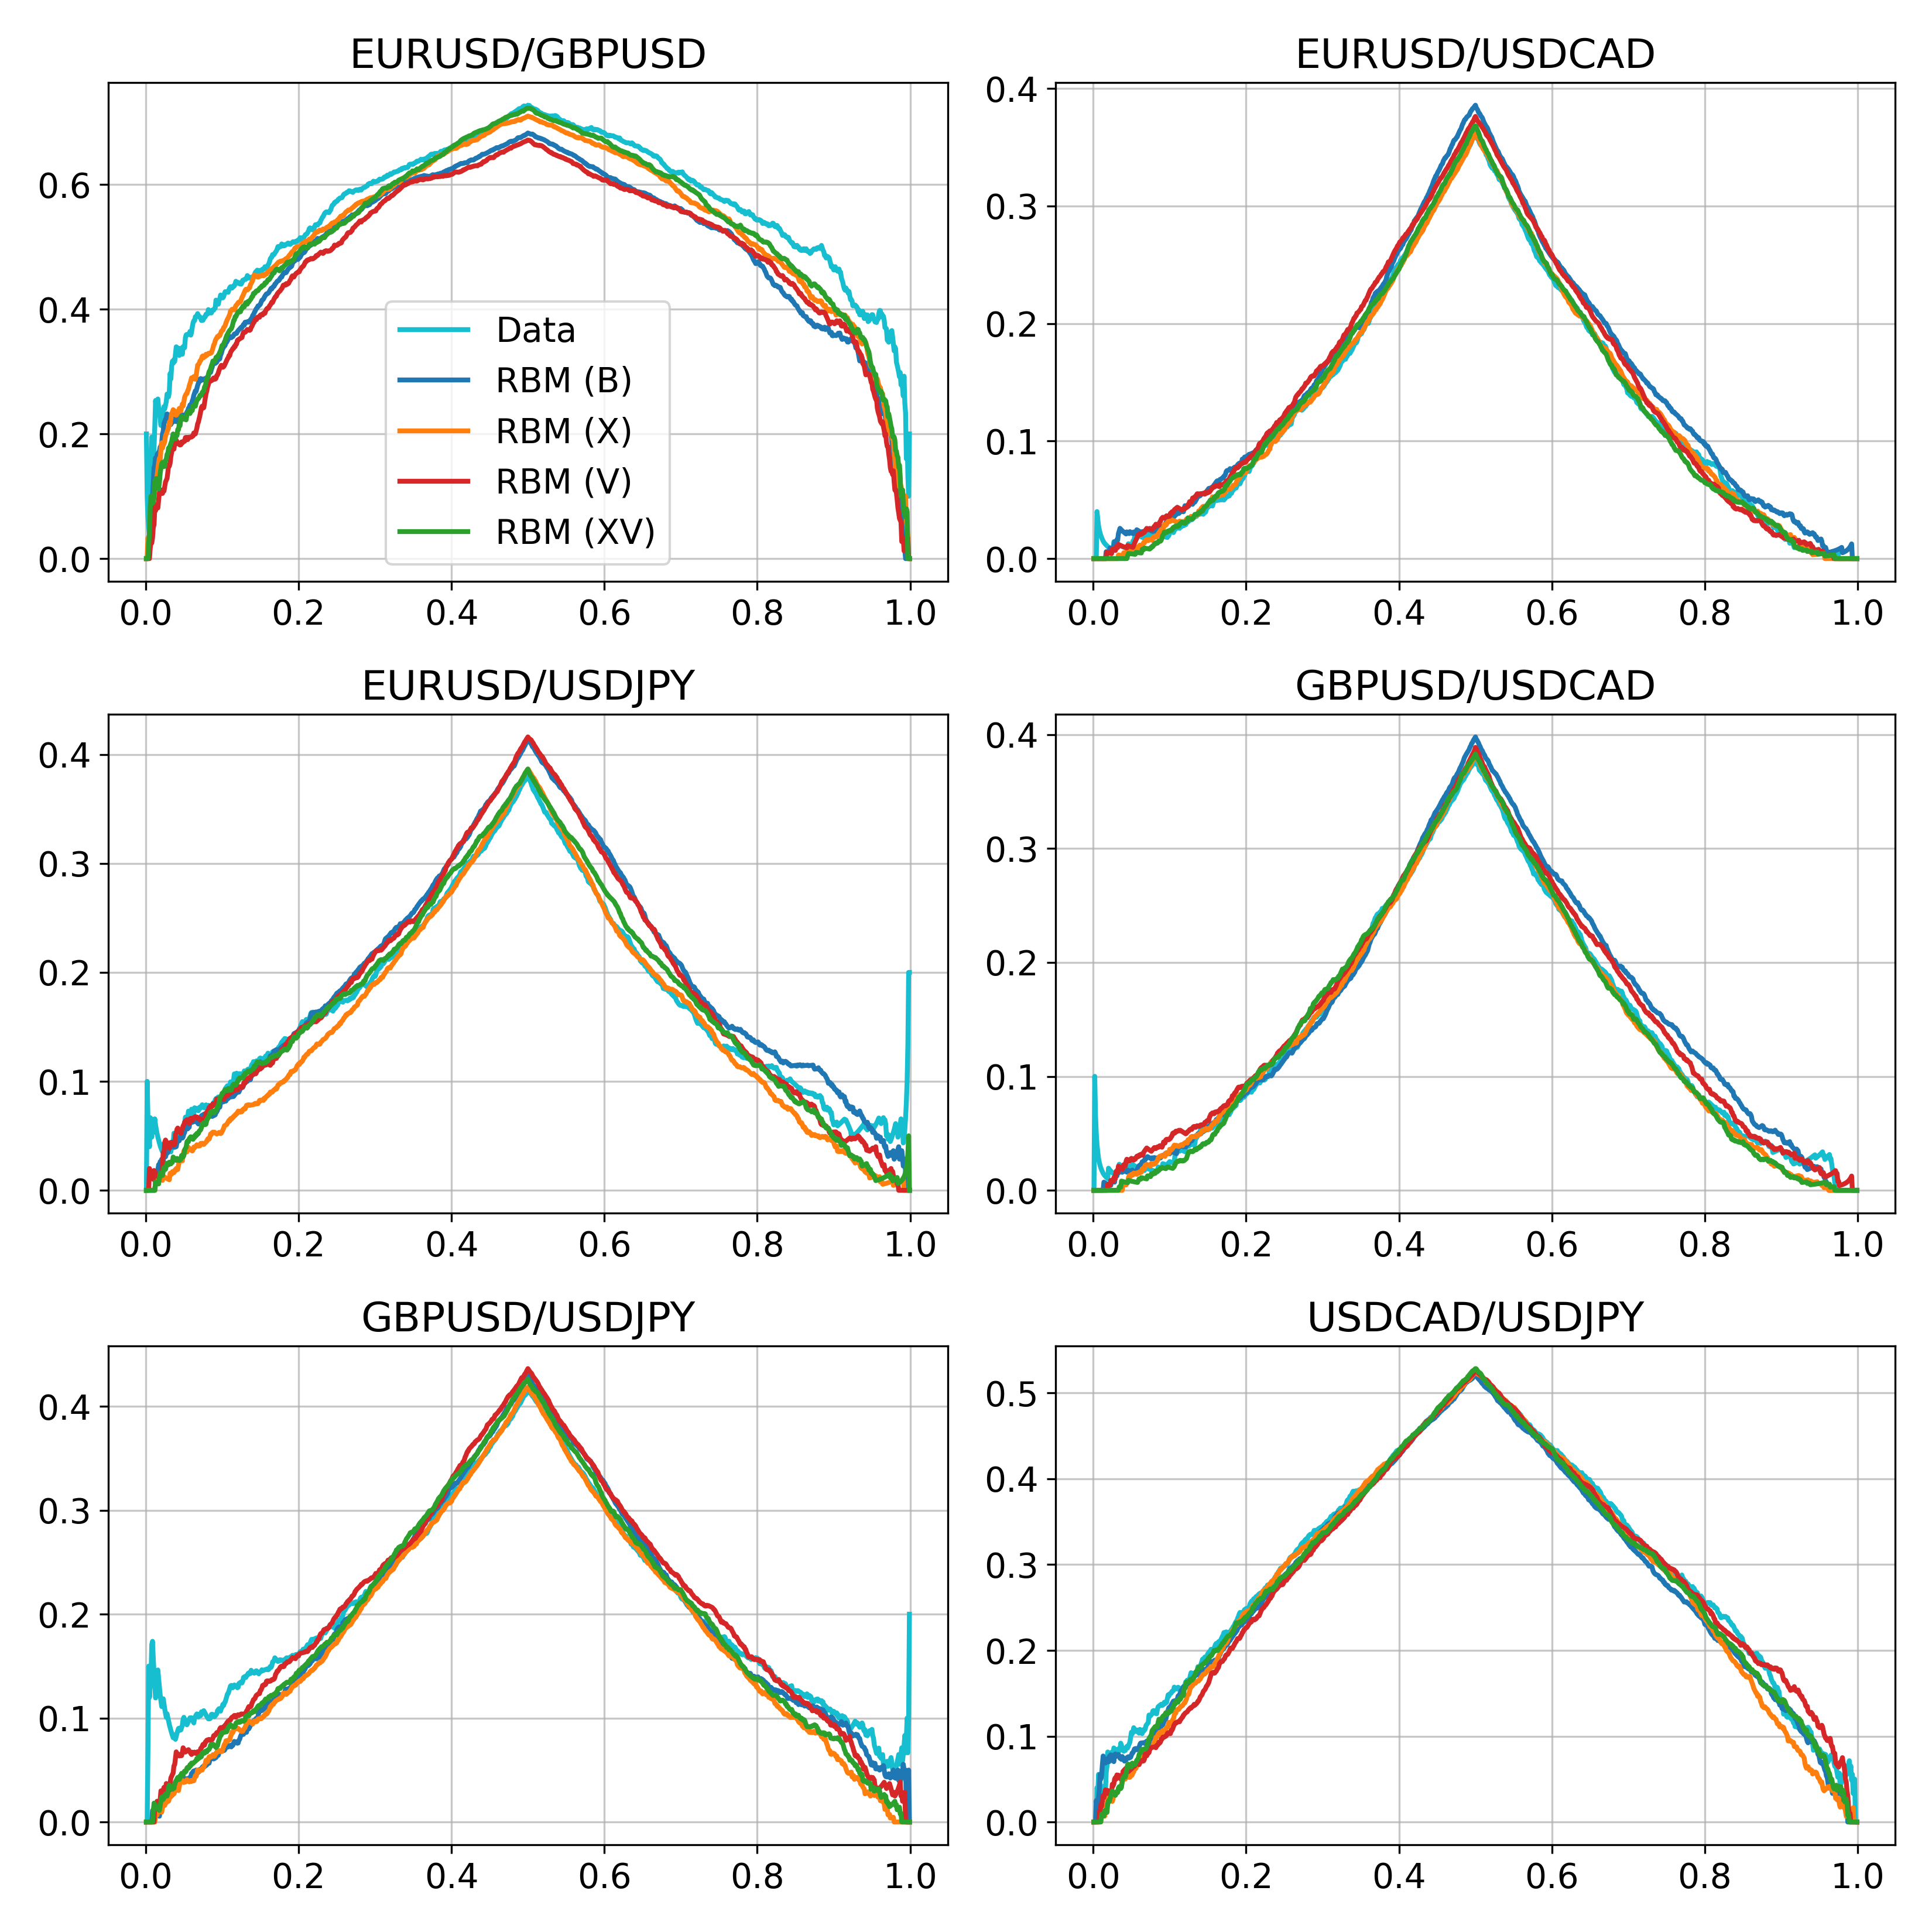
\includegraphics[width=1\linewidth]{rbm/tail_concentrations.png}
    \end{center}
    \caption{Tail concentration functions of the data vs. samples generated by the RBM models.}
    \label{fig:rbm_tail_concentrations}
\end{figure}

\begin{figure}[ht]
    \begin{center}
        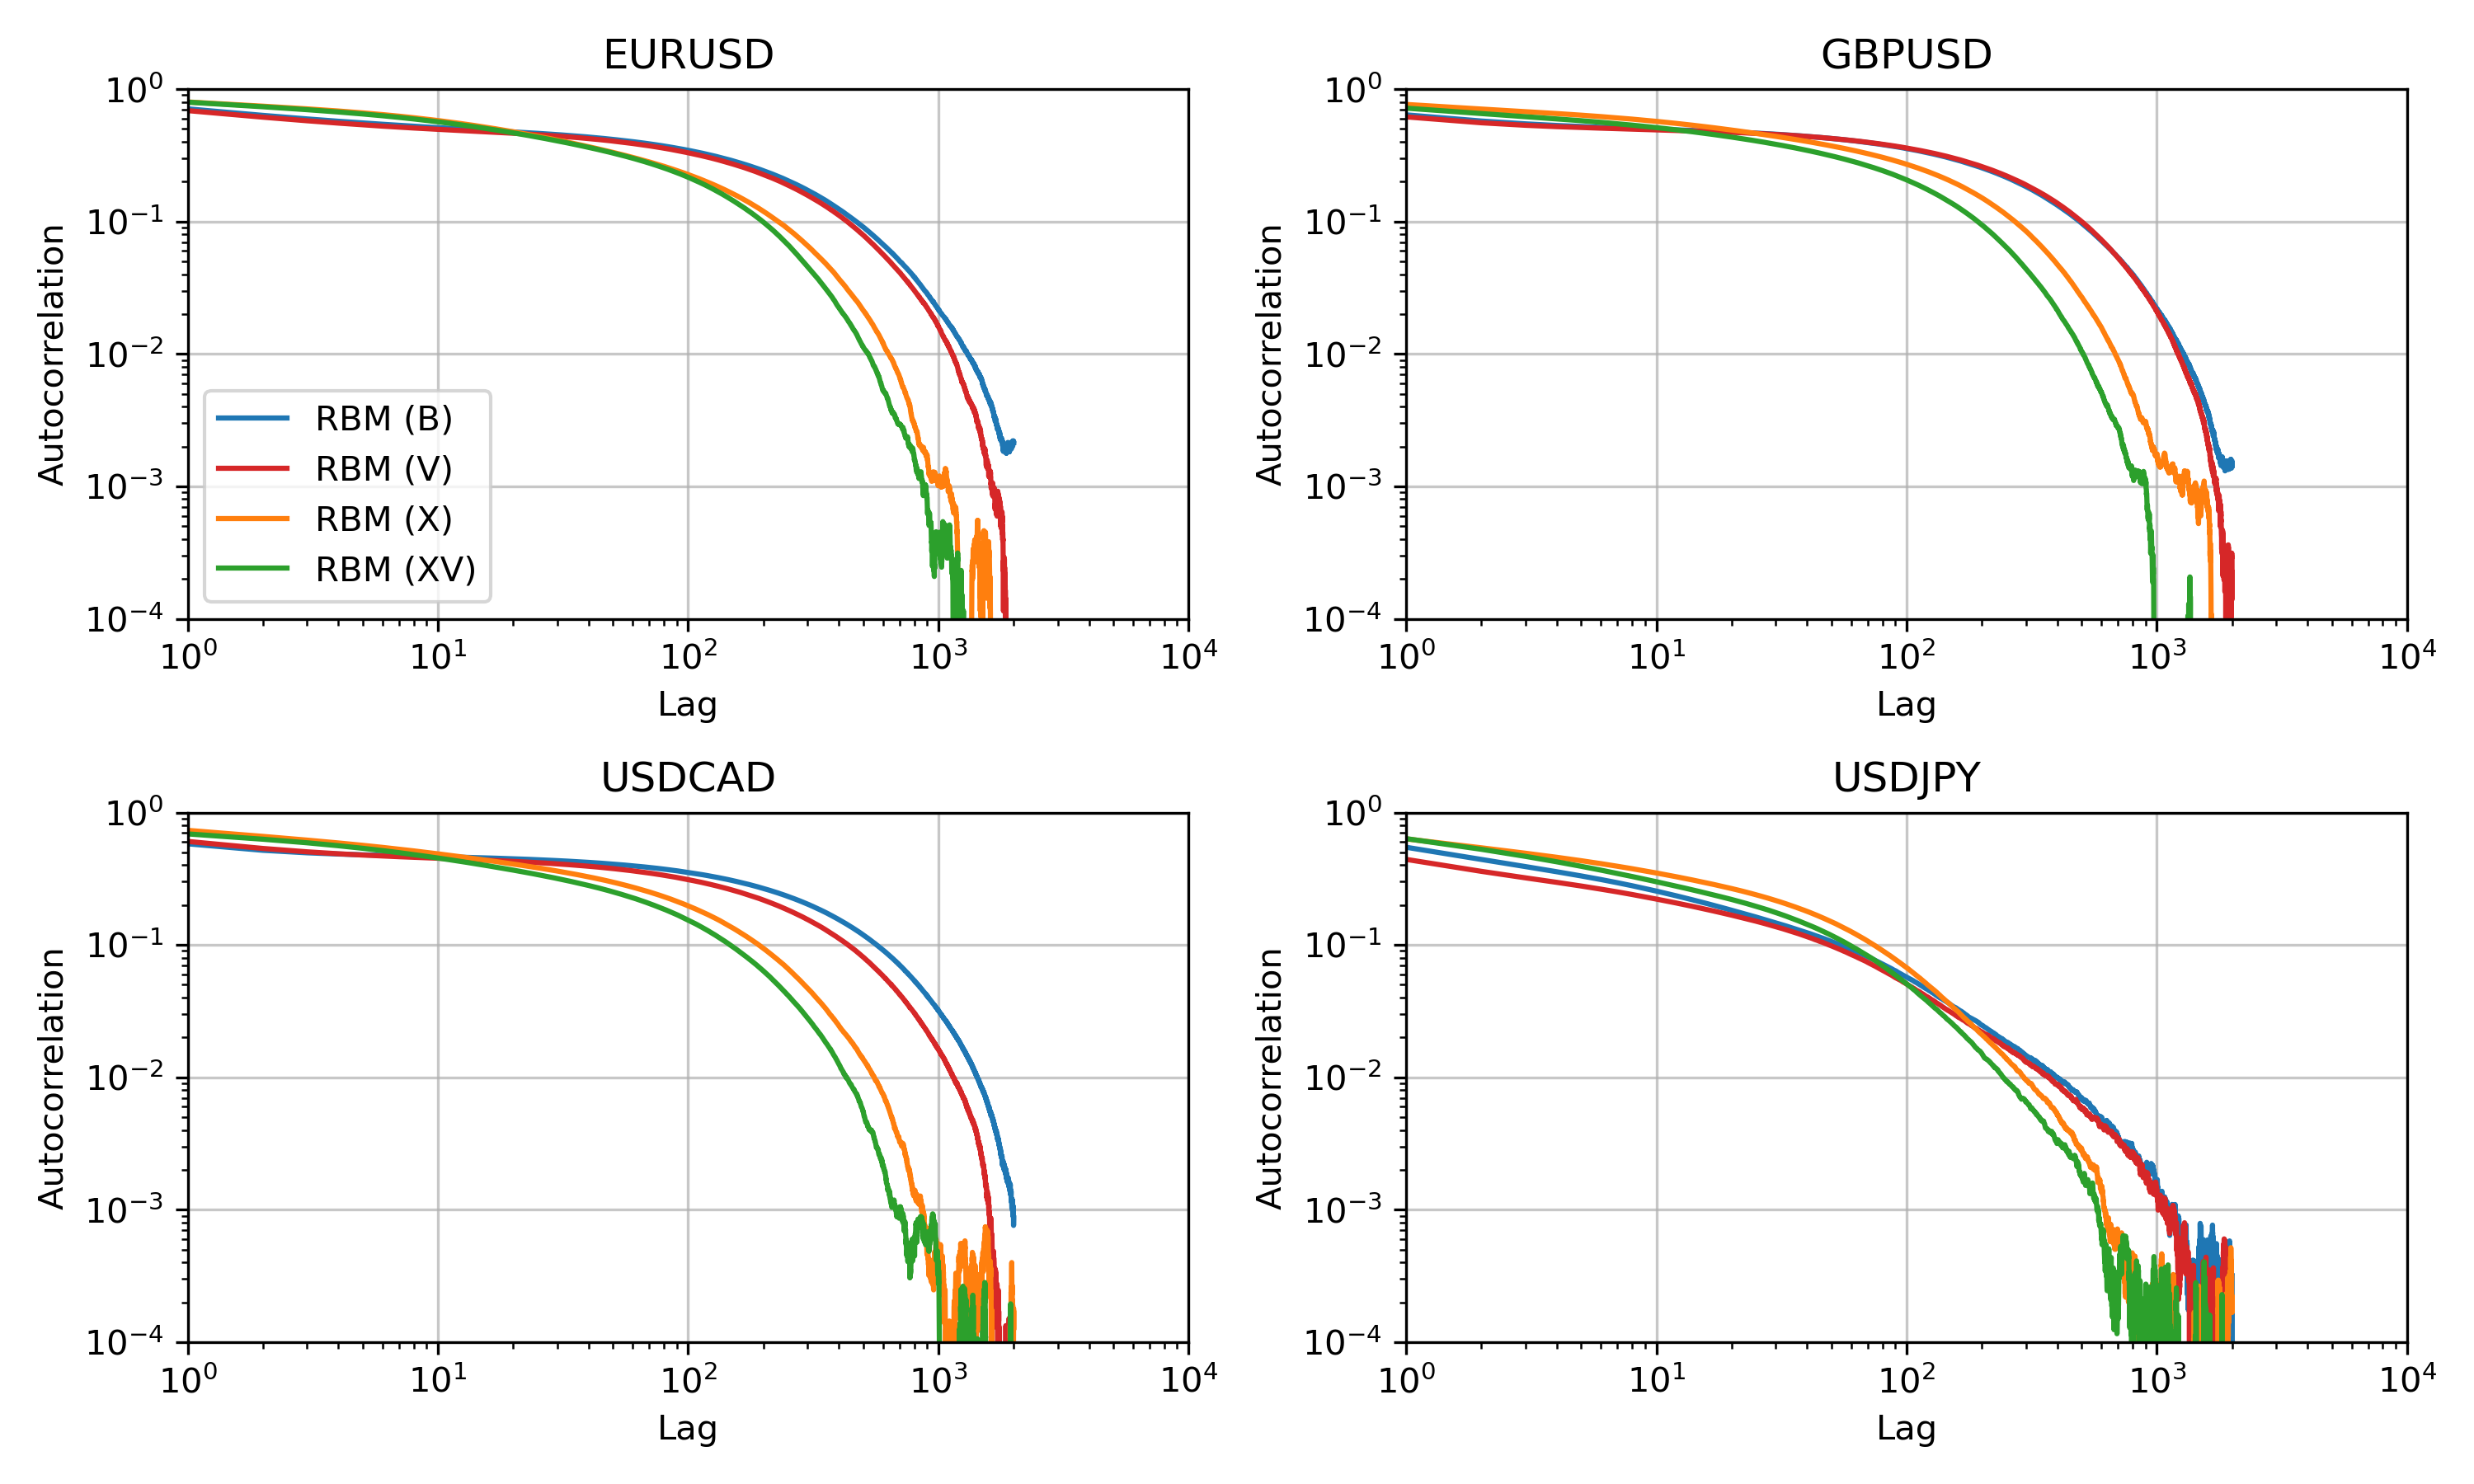
\includegraphics[width=1\linewidth]{rbm/autocorrelation_functions.png}
    \end{center}
    \caption{Autocorrelation functions of the RBM models. Function values are computed from Gibbs sample chains of length \( 10^8 \).}
    \label{fig:rbm_autocorrelation_functions}
\end{figure}

\begin{figure}[ht]
    \begin{center}
        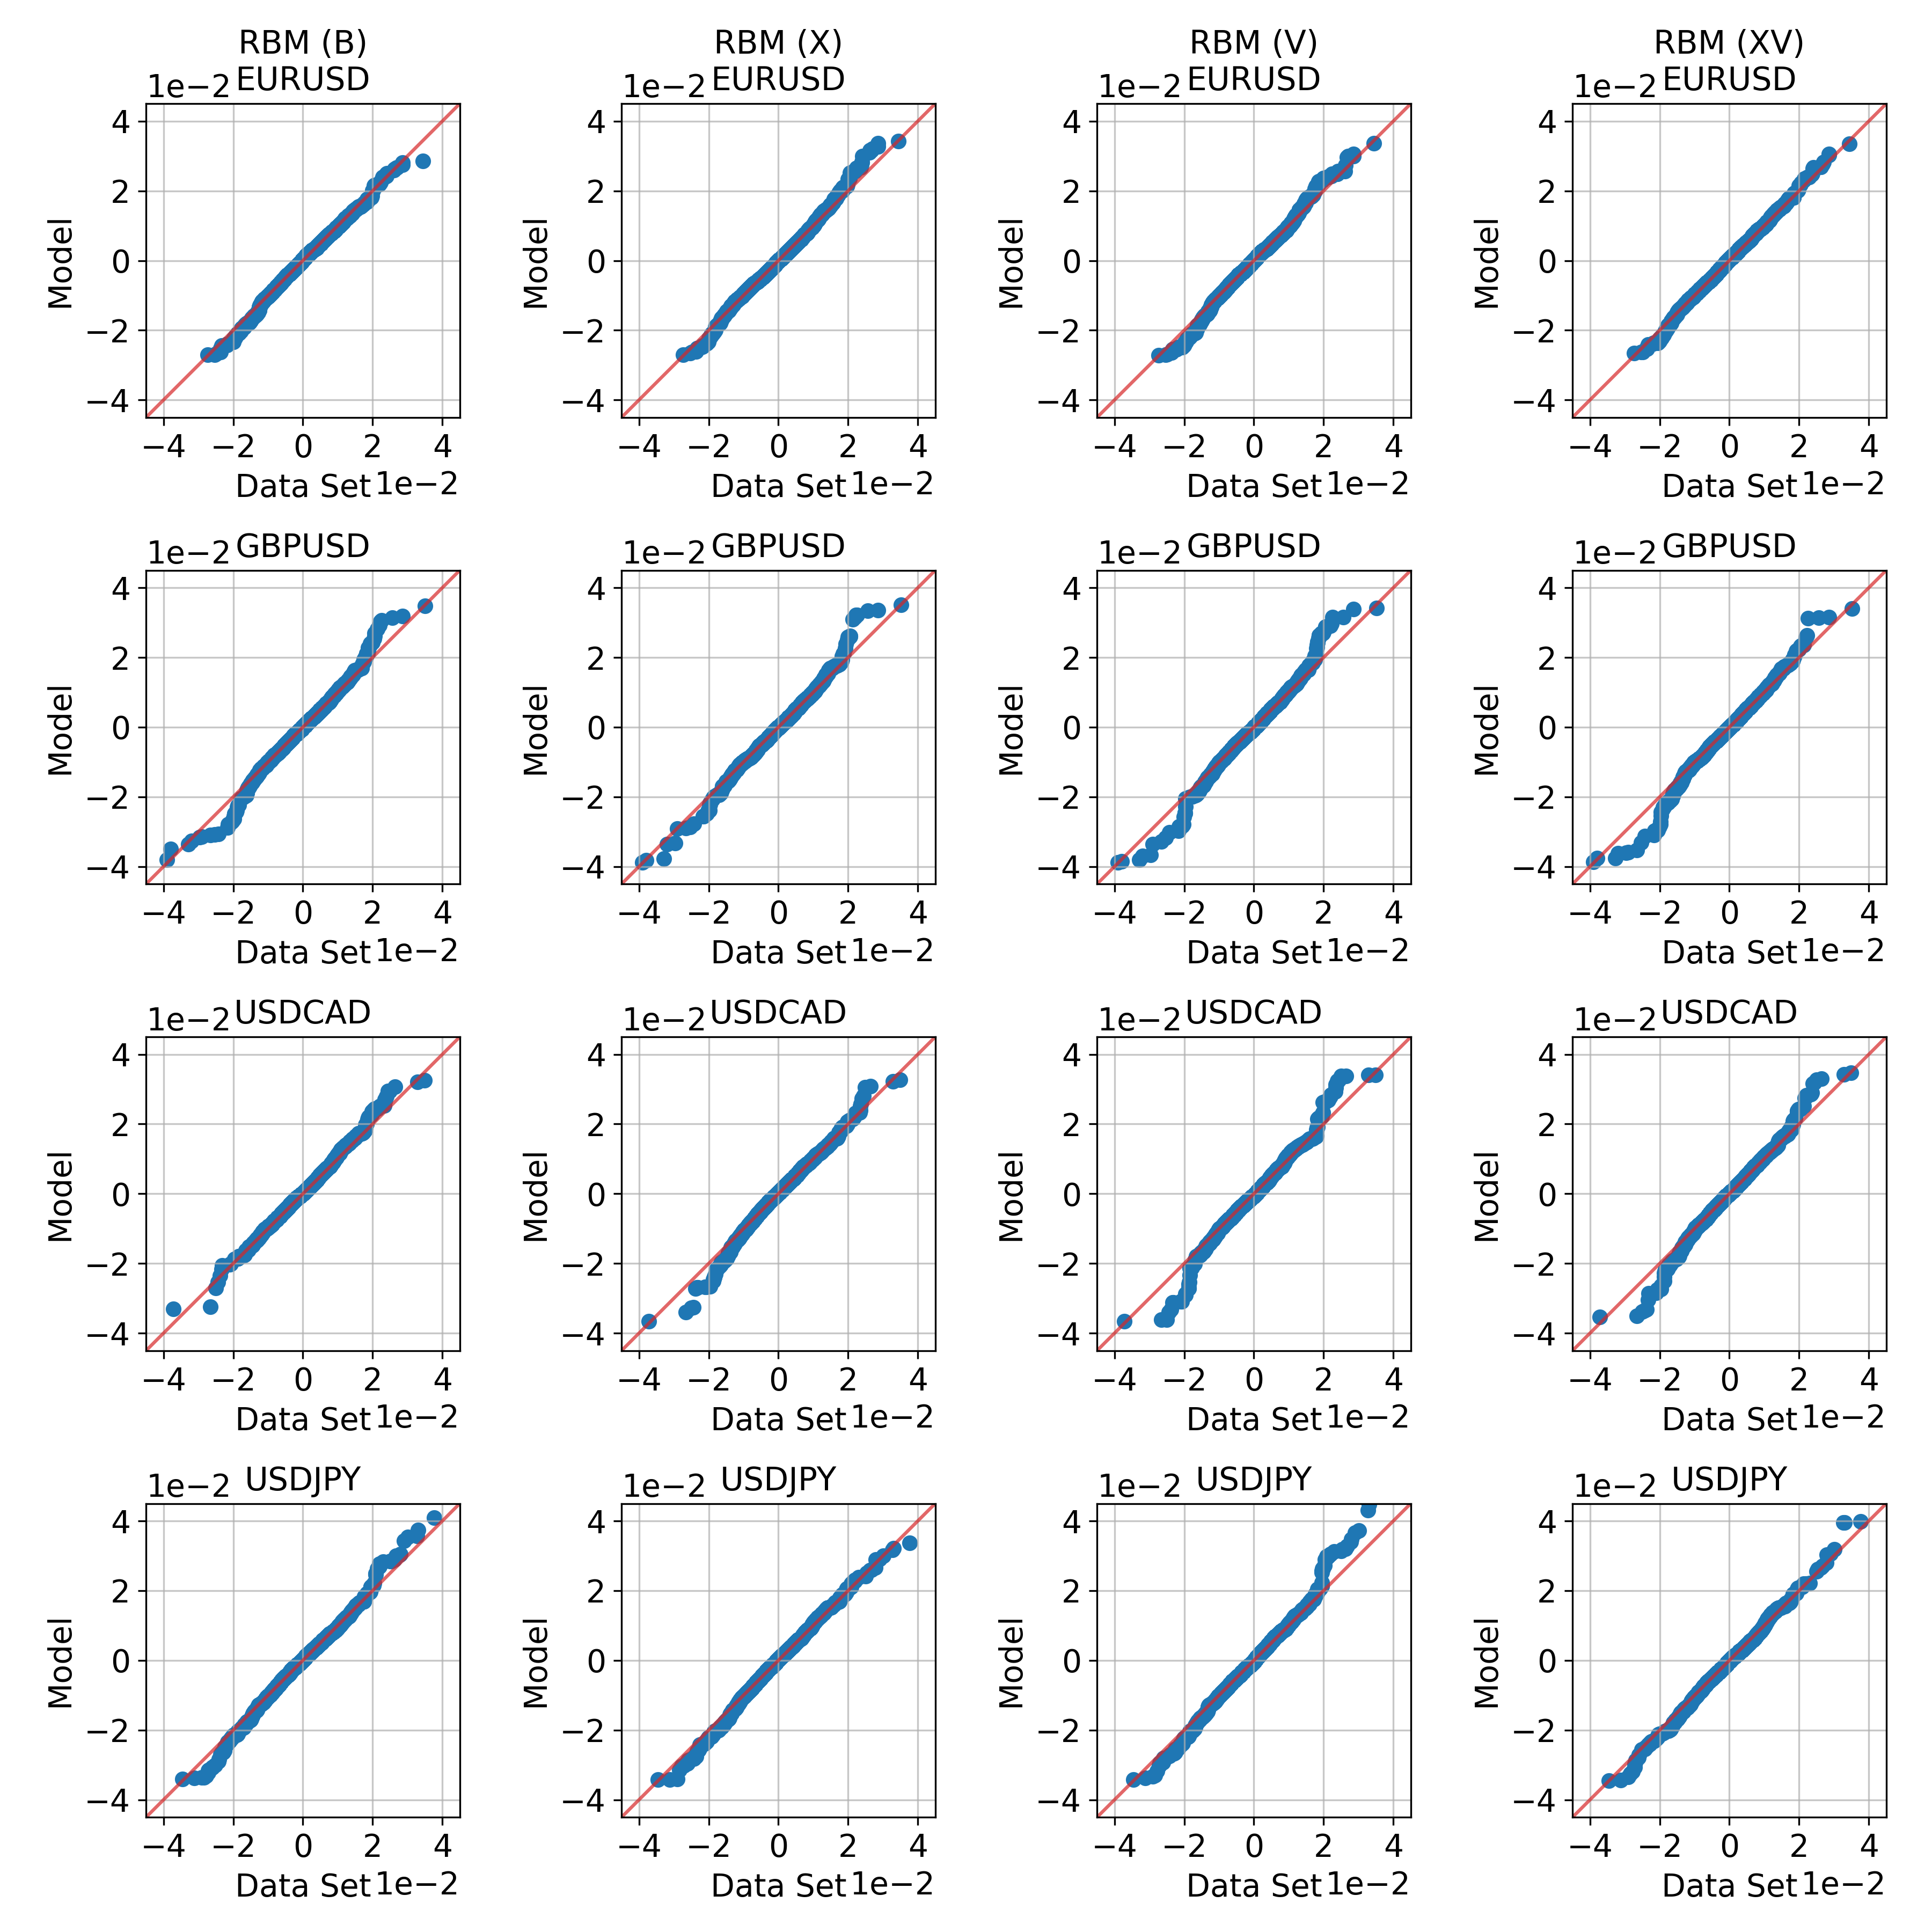
\includegraphics[width=1\linewidth]{rbm/qq.png}
    \end{center}
    \caption{QQ plots of the RBM models.}
    \label{fig:rbm_qq_plots}
\end{figure}


%----------------------------------------------------------------------------------------
% QBM
%----------------------------------------------------------------------------------------
\chapter{Quantum Boltzmann Machine}
\label{ch:qbm}
\section{Theory}
\todo{Quantum annealing theory}

\todo{Explain QUBO}

\section{Application}
\todo{D-Wave introduction/usage}

\section{Results}


%----------------------------------------------------------------------------------------
% Conclusion
%----------------------------------------------------------------------------------------
\chapter{Conclusion}
\label{ch:conclusion}
\section{Summary}
We started with an analysis of the forex log returns data set in~\cref{ch:data_analysis}, analyzing the data from a number of aspects to get an understanding of the intricacies.
After that, we moved to training classical RBM models in~\cref{ch:rbm}, where we were able to produce good results similar to those in~\cite{kondratyev_2019}.
The outlier power transformation detailed in~\cref{sec:outlier_transform} shows much promise, as models trained on the transformed data sets perform noticeably better than those trained on the base data sets.

After establishing a classical baseline to compare our quantum models with, we studied a small 12-qubit problem in~\cref{sec:qbm_12_qubit_problem}, through which we gained a deeper understanding of how to sample quantum Boltzmann random variables using a D-Wave quantum annealer, specifically the Advantage 4.1.
There, we were able to match sample distributions returned by the annealer to theoretical distributions from the family of distributions corresponding to the density operator \( \rho(s,T) = \frac{1}{Z}e^{-\beta H(s)} \).
Our findings indicate that, with the anneal schedules and parameters used here, the Advantage 4.1 is not able to sample from just any quantum Boltzmann distribution, rather only those that are classical Boltzmann-like in nature.
To be more specific, the samples we obtained from the annealer resemble a subset of the family of distributions that satisfies \( B(s) / T = \text{constant} \), as indicated by the streak patterns observed in~\cref{fig:dkl_min_heatmap}.
This occurs when the distribution is similar to one late in the anneal process, i.e., when \( e^{-\beta H(s^*)} \approx e^{-\beta B(s^*) H_\text{final}} \).
This is likely due to the annealer not being able to quench the system fast enough, allowing for nontrivial dynamics to occur, as the shortest allowed quench durations are still quite long relative to the qubit oscillation frequency in terms of gigahertz.
How closely the annealer can approximate a desired classical Boltzmann distribution was found to be dependent on both the embedding as well as the anneal schedule, thus it is highly recommended to tune these accordingly.

With the information that we can only reliably sample classical Boltzmann distributions, we moved to training a bound-based quantum restricted Boltzmann machine (BQRBM) with a freeze-out point of \( s^* = 1 \), essentially reducing the problem to a classical RBM trained using quantum assistance.
The difficulty of choosing the effective temperature was in this case easily circumvented by treating \( \beta \) as a learnable parameter as described in~\cref{sec:learning_beta} and verified in~\cref{sec:qbm_simulation_results}.
We trained BQRBM models using both a simulation and the Advantage 4.1 annealer, allowing us to compare exactly how close the Advantage 4.1-trained model is to the theory.
Additionally, we trained a classical RBM to use as a reference point.
In short, the BQRBM model trained using the Advantage 4.1 underperforms both the classical RBM as well as the simulation, as seen in~\cref{sec:qbm_annealer_results}.
The simulation-based model shows promise though, outperforming the classical RBM, offering hope for future annealer-trained models if annealers can further reduce the information loss associated with sampling (quantum) Boltzmann distributions.

Finally, we used the knowledge gained about how to train a small BQRBM and applied it to training a larger one in~\cref{sec:quantum_market_generator} using the log returns data set, mapping 94 logical qubits to 398 physical qubits with chain lengths of up to 7.
This model proved to be more challenging to train because setting the annealer hyperparameters (chain strength, anneal schedule, and embedding) can not be done as in the 12-qubit problem due to the fact that we can not simulate such a large system.
In practice, we had to choose these values by doing a limited hyperparameter scan, which was difficult due to increased training times that averaged around 15 minutes per epoch.
Longer epoch times originated from a combination of solver load and latency from Europe to the North American West Coast.
This meant that training a model for 100 epochs would have taken around a day, and if we wanted to fully train the models for all hyperparameters in our scan it would have taken weeks.

The results in~\cref{sec:qbm_log_returns_results} show that the BQRBM was able to learn to produce synthetic data similar to the log returns data set distribution to some extent, but drastically underperforms the classical RBM.
This could likely have been improved with a more exhaustive hyperparameter scan, but that was not necessarily feasible given the time requirements, and it is unclear if the results would have been significantly better given that even the 12-qubit BQRBM trained on the annealer underperforms the classical RBM.

In this thesis we laid out a framework with which one can train quantum Boltzmann machines using both simulations and D-Wave quantum annealers.
As part of this thesis, the Python package \texttt{qbm}~\cite{qbm} was developed to make it easy to train and study QBMs.
This package is open source and available to the public to encourage further study of QBMs.

Overall, this thesis furthered not only our understanding of QBMs, but that of D-Wave annealer sampling in general.
We hope that this work will be useful for future research and development.

\section{Future Directions}
Throughout this thesis we came across several directions which we would have liked to explore more in depth but did not have the time to.

It would be interesting to investigate if adding technical indicators to the log returns data set could increase model performance.
Given that the log returns data set used here only takes into account the currency pairs' behavior over one day (excluding the volatility indicators), technical indicators calculated using data over a historical window could enrich the data set with vital information to help the model better learn the complexities of the distribution.

The discretization procedure for converting continuous data into bit vectors could probably be further improved.
As we saw in~\cref{sec:classical_market_generator}, the models that used the outlier power-transformed data sets generate samples with lower KL divergences and better reproduced the correlations between the currency pairs.

Of most interest is simulating the time-dependent Schr\"odinger equation of the D-Wave annealer to determine how fast the system needs to quench in order to freeze out the dynamics.
This would give a good indication of how much quantum annealers need to improve in order to be able to sample from arbitrary quantum Boltzmann distributions.

Studying additional anneal schedule formats would also be a very interesting direction.
Reverse annealing was tested to a very small extent here only to see if it produced drastically different results than forward annealing, but was left out of the final research because the results did not show any significant improvements and led to added complexity due to the need to choose what state the system was initialized in and if the system was reinitialized to the same state after each measurement or not.


%----------------------------------------------------------------------------------------
% Appendix
%----------------------------------------------------------------------------------------
\appendix
\chapter{Appendix}
\label{ch:appendix}
\section{Restricted Boltzmann Machine}
\subsection{Conditional Probabilities}\label{app:conditional_probabilities_derivation}
This derivation follows along the lines of that found on p. 658-659 of~\cite{goodfellow_deep_learning}.
We start by noting
\begin{align}
    p(\vec{v,h}) = \frac{1}{Z} e^{-E(\vec{v},\vec{h})}.
\end{align}
From this we can derive the conditional probability
\begin{align}
\begin{split}
    p(\vec{h} | \vec{v})
        &= \frac{p(\vec{v},\vec{h})}{p(\vec{v})} \\
        &= \frac{1}{p(\vec{v})} \frac{1}{Z} \exp( \vec{a}^\intercal\vec{v} + \vec{b}^\intercal\vec{h} + \vec{v}^\intercal\mat{W}\vec{h} ) \\
        &= \frac{1}{Z'} \exp\bigg( \sum_j b_j h_j + \sum_j (\vec{v}^\intercal\mat{W})_j h_j \bigg) \\
        &= \frac{1}{Z'} \prod_j \exp\big( b_j h_j + (\vec{v}^\intercal\mat{W})_j h_j \big),
\end{split}
\end{align}
where
\begin{align}
    Z' = \sum_\vec{h} \exp( \vec{b}^\intercal\vec{h} + \vec{v}^\intercal\mat{W}\vec{h} ).
\end{align}
This leads us to
\begin{align}
\begin{split}
    p(h_j = 1 | \vec{v})
        &= \frac{\tilde{p}(h_j = 1 | \vec{v})}{\tilde{p}(h_j = 0 | \vec{v}) + \tilde{p}(h_j = 1 | \vec{v})} \\
        &= \frac{\exp\big( b_j + (\vec{v}^\intercal\mat{W})_j \big)}{1 + \exp\big( b_j + (\vec{v}^\intercal\mat{W})_j \big)} \\
        &= \sigma\big( b_j + (\vec{v}^\intercal\mat{W})_j \big).
\end{split}
\end{align}
Finally, we have
\begin{align}
    p(\vec{h} | \vec{v}) = \prod_j \sigma\big( (2\vec{h} - 1) \odot (\vec{b} + \mat{W}^\intercal\vec{v}) \big)_j.
\end{align}

Analogously for \( p(\vec{v} | \vec{h}) \) one finds
\begin{align}
    p(\vec{v} | \vec{h}) = \prod_i \sigma\big( (2\vec{v} - 1) \odot (\vec{a} + \mat{W}\vec{h}) \big)_i.
\end{align}

\subsection{Log-Likelihood Derivative}\label{app:rbm_log_likelihood_derivation}
For data set distribution \( p_\text{data} \) and parameters \( \theta = (\mat{W}, \vec{a}, \vec{b}) \) the average log-likelihood is given by
\begin{align}
\begin{split}
    \ell(\theta)
        &= \sum_{\vec{v}} p_{\text{data}}(\vec{v}) \log p(\vec{v}) \\
        &= \sum_{\vec{v}} p_{\text{data}}(\vec{v}) \log \sum_\vec{h} p(\vec{v},\vec{h}) \\
        &= \sum_{\vec{v}} p_{\text{data}}(\vec{v}) \log \bigg(\frac{1}{Z} \sum_\vec{h} e^{-E(\vec{v},\vec{h})}\bigg) \\
        &= \sum_{\vec{v}} p_{\text{data}}(\vec{v}) \log \sum_\vec{h} e^{-E(\vec{v},\vec{h})} - \log \sum_{\vec{v},\vec{h}} e^{-E(\vec{v},\vec{h})}.
\end{split}
\end{align}
Taking the gradient we find
\begin{align}
\begin{split}
    \partial_{\theta} \ell(\theta)
        &= \sum_{\vec{v}} p_{\text{data}}(\vec{v}) \frac{\sum_\vec{h} e^{-E(\vec{v},\vec{h})} \partial_{\theta}\big( -E(\vec{v},\vec{h}) \big) }{\sum_\vec{h} e^{-E(\vec{v},\vec{h})}}
            - \frac{\sum_{\vec{v},\vec{h}} e^{-E(\vec{v},\vec{h})} \partial_{\theta}\big( -E(\vec{v},\vec{h}) \big) }{\sum_{\vec{v},\vec{h}} e^{-E(\vec{v},\vec{h})}} \\
        &= \sum_{\vec{v}} p_{\text{data}}(\vec{v}) \Big\langle \partial_{\theta}\big( -E(\vec{v},\vec{h}) \big) \Big\rangle_{p(\vec{h}|\vec{v})}
        - \Big\langle \partial_{\theta}\big( -E(\vec{v},\vec{h}) \big) \Big\rangle_{p(\vec{v},\vec{h})},
\end{split}
\end{align}
where \( \langle \ \cdot \ \rangle_{\text{data}} \) denotes the expectation value with respect to the data set distribution, and \( \langle \ \cdot \ \rangle_{\text{model}} \) denotes the expectation value with respect to the model distribution.
This gives us
\begin{align}
\begin{split}
    \partial_{w_{ij}} \ell(\theta)
        &= \langle v_i h_j \rangle_{\text{data}} - \langle v_i h_j \rangle_{\text{model}}, \\
    \partial_{a_i} \ell(\theta)
        &= \langle v_i \rangle_{\text{data}} - \langle v_i \rangle_{\text{model}}, \\
    \partial_{b_j} \ell(\theta)
        &= \langle h_j \rangle_{\text{data}} - \langle h_j \rangle_{\text{model}}.
\end{split}
\end{align}

\section{Quantum Boltzmann Machine}
\subsection{Log-Likelihood Derivative}\label{app:qbm_log_likelihood_derivation}
This derivation follows along the lines of that laid out in~\cite{amin_2018}.
We start with the data set-averaged log-likelihood
\begin{align}
\begin{split}
    \ell(\theta)
        &= \sum_{\vec{v}} p_{\text{data}}(\vec{v}) \log p(\vec{v}) \\
        &= \sum_{\vec{v}} p_{\text{data}}(\vec{v}) \log \frac{\tr(\Lambda_\vec{v} e^{-H})}{\tr(e^{-H})} \\
        &= \sum_{\vec{v}} p_{\text{data}}(\vec{v}) \Big[ \log\tr(\Lambda_\vec{v} e^{-H}) - \log\tr(e^{-H}) \Big].
\end{split}
\end{align}
Taking the partial derivative yields
\begin{align}
    \label{eq:qbm_log_likelihood_derivative}
    \partial_\theta \ell(\theta)
        &= \sum_{\vec{v}} p_{\text{data}}(\vec{v}) \bigg[ \frac{\tr(\Lambda_\vec{v} \partial_\theta e^{-H})}{\tr(\Lambda_\vec{v} e^{-H})} - \frac{\tr(\partial_\theta e^{-H})}{\tr(e^{-H})} \bigg].
\end{align}
Due to the noncommutativity of \( H \) and \( \partial_\theta H \), we need to use the trick laid out in~\cite{amin_2018} where we take \( e^{-H} = (e^{-\delta\tau H})^n \) with \( \delta\tau \equiv 1 / n \), which allows one to write
\begin{align}
    \partial_\theta e^{-H}
        &= -\sum_{m=1}^{n} e^{-m\delta\tau H} \delta\tau \partial_\theta He^{-(n-m)\delta\tau H} + \mathcal{O}(\delta\tau^2).
\end{align}
Taking the limit as \( n \rightarrow \infty \) of both sides gives
\begin{align}
\begin{split}
    \partial_\theta e^{-H}
        &= \lim_{n\rightarrow\infty} -\sum_{m=1}^{n} e^{-m\delta\tau H} \delta\tau \partial_\theta He^{-(n-m)\delta\tau H} + \mathcal{O}(\delta\tau^2) \\
        &= -\int_{0}^{1} d\tau e^{-\tau H} \partial_\theta H e^{(\tau-1)H}.
\end{split}
\end{align}
From here one can take the trace of both sides to arrive at
\begin{align}
\begin{split}
    \tr(\partial_\theta e^{-H})
        &= -\tr\bigg( \int_{0}^{1} d\tau e^{-\tau H} \partial_\theta H e^{(\tau-1)H} \bigg) \\
        &= -\int_{0}^{1} d\tau \tr\big(e^{-\tau H} \partial_\theta H e^{(\tau-1)H} \big) \\
        &= -\int_{0}^{1} d\tau \tr\big(e^{(\tau-1)H} e^{-\tau H} \partial_\theta H \big) \\
        &= -\int_{0}^{1} d\tau \tr\big(e^{-H} \partial_\theta H \big) \\
        &= -\tr\big(e^{-H} \partial_\theta H \big),
\end{split}
\end{align}
which gives
\begin{align}
\begin{split}
    \frac{\tr(\partial_\theta e^{-H})}{\tr(e^{-H})}
        &= -\frac{\tr(e^{-H} \partial_\theta H)}{\tr(e^{-H})} \\
        &= -\tr(\rho \partial_\theta H) \\
        &= -\langle \partial_\theta H \rangle.
\end{split}
\end{align}
Unfortunately, due to the additional factor of \( \Lambda_\vec{v} \) in the first term of \cref{eq:qbm_log_likelihood_derivative}, one arrives at
\begin{align}
\begin{split}
    \tr(\Lambda_\vec{v} \partial_\theta e^{-H})
        &= -\tr\bigg( \int_{0}^{1} d\tau \Lambda_\vec{v} e^{-\tau H} \partial_\theta H e^{(\tau-1)H} \bigg) \\
        &= -\int_{0}^{1} d\tau \tr\big(\Lambda_\vec{v} e^{-\tau H} \partial_\theta H e^{(\tau-1)H} \big),
\end{split}
\end{align}
which is nontrivial to compute in practice.

\subsection{Log-Likelihood Lower Bound}\label{app:qbm_log_likelihood_lower_bound}
This derivation follows along the lines of that laid out in~\cite{amin_2018}.
The Golden-Thompson inequality that \( \tr(e^{A}e^{B}) \ge \tr(e^{A+B}) \) allows one to write (for small \( \epsilon > 0 \))
\begin{align}
    \tr(e^{-H} e^{\log(\Lambda_\vec{v}+\epsilon)}) \ge \tr(e^{-H+\log(\Lambda_\vec{v}+\epsilon)}).
\end{align}
Taking the limit \( \epsilon \rightarrow 0 \) yields
\begin{align}
    \tr(\Lambda_\vec{v}e^{-H}) \ge \tr(e^{-H_\vec{v}}),
\end{align}
where
\begin{align}
    H_\vec{v} &= \braket{\vec{v} | H | \vec{v}},
\end{align}
with \( H_\vec{v} \) being the \textit{clamped} Hamiltonian.
This is called clamped because the visible qubits are held to the classical state of the visible vector \( \vec{v} \) due to an infinite energy penalty imposed by the \( \log(\Lambda_\vec{v} + \epsilon) \) term.
Using this we can write the inequality
\begin{align}
\begin{split}
    p(\vec{v})
        &= \frac{\tr(\Lambda_\vec{v} e^{-H})}{\tr(e^{-H})} \\
        &\ge \frac{\tr(e^{-H_\vec{v}})}{\tr(e^{-H})},
\end{split}
\end{align}
which in turn allows for the log-likelihood to be bounded as
\begin{align}
    \ell(\theta) \ge \tilde{\ell}(\theta),
\end{align}
where
\begin{align}
    \tilde{\ell}(\theta)
        &= \sum_\vec{v} p_\text{data}(\vec{v}) \log\frac{\tr(e^{-H_\vec{v}})}{\tr(e^{-H})}.
\end{align}
\subsection{Log-Likelihood Lower Bound Derivative}\label{app:qbm_log_likelihood_lower_bound_derivative}
This derivation follows along the lines of that laid out in~\cite{amin_2018}.
Taking the partial derivative of the log-likelihood lower bound yields
\begin{align}
\begin{split}
    \label{eq:qbm_log_likelihood_derivative_lower_bound}
    \partial_\theta \tilde{\ell}(\theta)
        &= \sum_{\vec{v}} p_{\text{data}}(\vec{v}) \bigg[ \frac{\tr(\partial_\theta e^{-H_\vec{v}})}{\tr(e^{-H_\vec{v}})} - \frac{\tr(\partial_\theta e^{-H})}{\tr(e^{-H})} \bigg] \\
        &= \sum_{\vec{v}} p_{\text{data}}(\vec{v}) \bigg[ \frac{\tr(e^{-H_\vec{v}} \partial_\theta H_\vec{v})}{\tr(e^{-H_\vec{v}})} - \frac{\tr(e^{-H} \partial_\theta H)}{\tr(e^{-H})} \bigg] \\
        &= \sum_{\vec{v}} p_{\text{data}}(\vec{v}) [ \tr(\rho_\vec{v} \partial_\theta H_\vec{v}) - \tr(\rho \partial_\theta H) ] \\
        &= \sum_{\vec{v}} p_{\text{data}}(\vec{v}) [ \langle \partial_\theta H_\vec{v} \rangle_\vec{v} - \langle \partial_\theta H \rangle ] \\
        &= \overline{\langle \partial_\theta H_\vec{v} \rangle_\vec{v}} - \langle \partial_\theta H \rangle.
\end{split}
\end{align}
Plugging in our parameters we get
\begin{align}
\begin{split}
    \partial_{w_{ij}} \tilde{\ell}(\theta)
        &= \overline{\langle \sigma_i^z \sigma_j^z \rangle_\vec{v}} - \langle \sigma_i^z \sigma_j^z \rangle \\
        &= \langle \sigma_i^z \sigma_j^z \rangle_\text{data} - \langle \sigma_i^z \sigma_j^z \rangle_\text{model}, \\
    \partial_{b_i} \tilde{\ell}(\theta)
        &= \overline{\langle \sigma_i^z \rangle_\vec{v}} - \langle \sigma_i^z \rangle \\
        &= \langle \sigma_i^z \rangle_\text{data} - \langle \sigma_i^z \rangle_\text{model}.
\end{split}
\end{align}
When restrictions are imposed on connections within the hidden layer, the clamped Hamiltonian reduces to
\begin{align}
    H_\vec{v}
        &= -\sum_i \big(\Gamma_i \sigma_i^x + b_i'(\vec{v}) \sigma_i^z\big),
\end{align}
where \( b_i'(\vec{v}) = b_i + (\mat{W}^\intercal\vec{v})_i \).
This allows one to rewrite the clamped density matrix as
\begin{align}
\begin{split}
    \rho_\vec{v}
        &= \frac{1}{Z_\vec{v}} \exp\bigg( \sum_i \big(\Gamma_i \sigma_i^x + h_i'(\vec{v}) \sigma_i^z\big) \bigg) \\
        &= \frac{1}{Z_\vec{v}} \prod_i \exp \big(\Gamma_i \sigma_i^x + b_i'(\vec{v}) \sigma_i^z\big) \\
        &= \prod_i \rho_\vec{v}^{(i)}.
\end{split}
\end{align}
With this we can compute the expectation values as
\begin{align}
\begin{split}
    \langle \sigma_i^z \rangle_\vec{v}
        &= \tr(\rho_\vec{v}^{(i)}\sigma_i^z) \\
        &= \frac{\tr\bigg[ \exp \big(\Gamma_i \sigma_i^x + b_i'(\vec{v}) \sigma_i^z\big) \sigma_i^z \bigg]}{\tr\bigg[ \exp \big(\Gamma_i \sigma_i^x + b_i'(\vec{v}) \sigma_i^z\big) \bigg]} \\
        &= \frac{b_i'(\vec{v})}{D_i(\vec{v})} \tanh\big(D_i(\vec{v})\big),
\end{split}
\end{align}
where \( D_i(\vec{v}) = \sqrt{\Gamma_i^2 + b_i'(\vec{v})^2} \).

The last equality above is obtained by using that for traceless \( A \) with \( \det A < 0 \) we can write
\begin{align}
    \exp(A) = \cosh\Big(\sqrt{\abs{\det A}}\Big) I + \frac{1}{\sqrt{\abs{\det A}}}\sinh\Big(\sqrt{\abs{\det A}}\Big) A.
\end{align}
This is obtained by using Cayley-Hamilton theorem along with the series expansion of the matrix exponential and grouping the terms.

\subsection{Learning The Effective Inverse Temperature \( \beta \)}\label{app:learning_beta}
Following along the lines of~\cite{xu_2021} we have
\begin{align}
\begin{split}
    p_\text{DW}
        &= \frac{1}{Z_\text{DW}} e^{-E_\text{DW}} \\
        &= \frac{1}{Z_\text{DW}} e^{-E / \beta},
\end{split}
\end{align}
which leads to a log-likelihood derivative of
\begin{align}
    \frac{\partial \log p_\text{DW}}{\partial\beta}
        &= \frac{1}{\beta^2} (E - \langle E \rangle),
\end{align}
and after averaging over the training data set we have
\begin{align}
    \Delta\beta
        &= \frac{\eta}{\beta^2}\big(\langle E \rangle_\text{data} - \langle E \rangle_\text{model}\big).
\end{align}

\section{Miscellaneous}
\subsection{Annualized Volatility}\label{app:annualized_volatility}
In finance, the annualized volatility of a time series vector \( \vec{x} \) is computed as
\begin{align}
    \text{vol}(\vec{x}) = \sqrt{252} \cdot \text{std}(\vec{x}),
\end{align}
where the factor of \( \sqrt{252} \) comes from the square root of the number of trading days in a year, i.e., it's the annualization factor.

\subsection{KL Divergence}\label{app:kl_divergence}
The Kullback-Leibler divergence~\cite{kullback_1951} is a measure of how much the probability distribution \( q \) differs from the reference probability distribution \( p \).
It is defined as
\begin{align}
    \DKL{p}{q}
        &= \sum_{x} p(x) \log\frac{p(x)}{q(x)}.
\end{align}
It can be interpreted as the amount of information loss associated with using \( q \) to approximate \( p \).
It must also be noted that the KL divergence is a distance, but not a metric (rather a divergence), because of the asymmetry that \( \DKL{p}{q} \ne \DKL{q}{p} \).

\subsubsection{KL Divergence in Practice}\label{app:kl_divergence_in_practice}
Due to the limited maximum sample size of \( 10^4 \) when using a D-Wave annealer and the inability to concatenate sample sets due to spin-bath polarization effects~\cite{pochart_2021}, it made computation of the KL divergence quite difficult because we couldn't get a proper read on the probability distribution when the number of possible states was high.
Even for the small 12-qubit problem there were still \( 2^{12} = 4096 \) possible states, thus \( 10^4 \) samples weren't entirely representative of the true distribution.
This problem was only exacerbated when working with larger system sizes.

Therefore, in this thesis we chose to take a histogram-based approach to approximate the KL divergence.
All KL divergences were computed using 32 bins since this was close to the number of bins computed using the Freedman-Diaconis rule on some of the sample sets for the 12-qubit problem.

When computing the \( q \) distribution from a sample set of limited size, it was inevitable that some of the probabilities came out to zero, which in turn led to issues computing the KL divergence due to zeros in the denominator of the argument of the log.
Luckily there was a way around this if we knew the true probability of measuring such a state to be nonzero.
Due to the quantum nature of this problem and the fact that no state had a truly zero probability (although some infinitesimally small), we could take such an approach.

The method we used to mitigate this problem is called smoothing~\cite{han_kl_divergence}, where we added some small probability \( \epsilon \) to the \( q \) distribution probabilities that were observed to be zero, then took the sum of the added probabilities and evenly subtracted it from the nonzero probabilities in order to ensure the distribution remain normalized.
For example, if \( \{q_1 = 1/3, q_2 = 2/3, q_3 = 0, q_4 = 0\} \), then the smoothed distribution would be \( \{q_1 = 1/3 - \epsilon, q_2 = 2/3 - \epsilon, q_3 = \epsilon, q_4 = \epsilon\} \).

Furthermore, call it \textit{relative} smoothing when the smoothed probabilities were taken to be relative to the reference distribution \( p \), which was found to be useful when it was difficult to choose a constant value of \( \epsilon \), e.g. when the reference distribution probabilities varied widely and could sometimes coincide with \( \epsilon \).
For example, if \( \{q_1 = 1/3, q_2 = 2/3, q_3 = 0, q_4 = 0\} \), then the relative smoothed distribution would be \( \{q_1 = 1/3 - \epsilon (p_3 + p_4)/2, q_2 = 2/3 - \epsilon (p_3 + p_4)/2, q_3 = \epsilon p_3, q_4 = \epsilon p_4\} \).

We took a value of \( \epsilon = 10^{-6} \) when computing \( \DKL{\pdata}{\pmodel} \) because it was small enough that it wouldn't coincide with any of the \( \pdata \) values since the data sets contained only a few thousand samples, thus the smallest value of \( \pdata \) was roughly on the order of \( 10^{-4} \).
When computing \( \DKL{\ptheory}{\psamples} \) though, we opted to use relative smoothing with a value of \( \epsilon = 10^{-6} \) since sometimes some probabilities of \( \ptheory \) could be close to \( \epsilon \) and give a false sense of agreement with the smoothed \( \psamples \).

\subsection{Correlation Coefficients}\label{app:correlation_coefficients}
The Pearson correlation coefficient is defined as
\begin{align}
    \rho_{X,Y} = \frac{\text{cov}{(X,Y)}}{\sigma_X \sigma_Y} \in [-1, 1],
\end{align}
and measures the linear correlation between the random variables \( X \) and \( Y \).
Therefore, it must be noted that this does not capture nonlinear relations, and shouldn't be relied upon to tell the full story.
Additionally, this measure is quite sensitive to outliers.

The Spearman rank correlation coefficient is defined as
\begin{align}
    r_s = \rho_{R(X),R(Y)} = \frac{\text{cov}{\big(R(X),R(Y)\big)}}{\sigma_{R(X)} \sigma_{R(Y)}} \in [-1, 1],
\end{align}
and is the Pearson correlation coefficient of the rank of the random variables \( X \) and \( Y \).
The main difference to the Pearson correlation coefficient is that the Spearman measures the monotonic relationship, regardless of linearity.
The Spearman correlation coefficient is also less sensitive to outliers than the Pearson.

The Kendall rank correlation coefficient is defined as
\begin{align}
    \tau = \frac{2}{n(n-1)} \sum_{i<j} \text{sign}(x_i - x_j) \text{sign}(y_i - y_j) \in [-1, 1],
\end{align}
where \( (x_1, y_1), \dots, (x_n, y_n) \) are pairs of observations of the random variables \( X \) and \( Y \).

It is important to keep in mind how one interprets the correlation coefficients.
The sign of the correlation coefficient determines whether or not it is negatively or positively correlated, and the magnitude determines how strong the correlation effects are.
As a loose guide, correlation coefficient values of 0.1, 0.3, and 0.5 can be termed small, medium, and large, respectively~\cite{research_design_and_statistical_analysis}.
In general, one must be careful when interpreting the correlation coefficients; it is important to understand what the values mean, and what they don't.
Section 3.4.2 "Interpreting the Correlation Coefficient" of~\cite{research_design_and_statistical_analysis} offers further insight and points out some of the pitfalls to watch out for.

In this thesis the correlation coefficients were computed using the respective functions from the SciPy Python package~\cite{python_scipy}.

\subsection{Tail Concentration Functions}\label{app:tail_concentration_functions}
The lower tail concentration function is defined as~\cite{venter_2002}
\begin{align}
\begin{split}
    L(z)
        &= \frac{p(U_1 \le z, U_2 \le z)}{z} \\
        &= \frac{C(z,z)}{z},
\end{split}
\end{align}
and the upper as
\begin{align}
\begin{split}
    R(z)
        &= \frac{p(U_1 > z, U_2 > z)}{1-z} \\
        &= \frac{1 - 2z + C(z,z)}{1-z},
\end{split}
\end{align}
where \( U_1 \) and \( U_2 \) uniform random variables on the interval \( [0, 1] \), and \( C(u_1, u_2) \) is the copula of \( (U_1, U_2) \).

In practice we computed \( U_1 \) and \( U_2 \) as the normalized rank of the observations of the random variables \( X \) and \( Y \), respectively.
The way to interpret the concentration functions is that they represent the probability that \( X \) and \( Y \) simultaneously take on extreme values.
When plotted, the lower tail concentration function is used for \( 0 \le z \le 0.5 \) and the upper for \( 0.5 \le z \le 1 \).

A nice explanation with animations can be found at~\cite{charpentier_2012}.

\subsection{Autocorrelation Analysis}\label{app:autocorrelation_analysis}
When studying results from an MCMC-based model it is important to be aware that sequentially generated samples are not always statistically independent, that is, there is some thermalization threshold that corresponds to the minimum number of sampling steps between samples to consider them as statistically independent.

For a time series \( x_1, \dots, x_n \), the lag-\( k \) autocorrelation function is defined as~\cite{time_series_analysis}
\begin{align}
    \rho_k
        &= \frac{\text{cov}(x_t, x_{t+k})}{\sigma_{x}^2}.
\end{align}
The autocorrelation function is essentially a correlation coefficient, except instead of comparing two different variables it compares the same variable at different times.
In this thesis we used the statsmodels Python package~\cite{python_statsmodels} to compute the autocorrelation function as there are some caveats when computing it in practice with large chains, e.g. there are some tricks such as using a Fourier transformation to make the computations more efficient.

The integrated autocorrelation time is a reasonable estimate of how many steps in between samples we should have before we can consider them to be (to a degree) statistically independent.
In this thesis we used the emcee Python package~\cite{python_emcee} to estimate the integrated autocorrelation time, which follows the approach laid out by Goodman and Weare in~\cite{goodman_weare_2010}.

\subsection{Exact Computation of \( \rho \)}\label{app:exact_rho_computation}
For the density matrix
\begin{align}
    \rho = \frac{1}{Z} e^{-\beta H},
\end{align}
we can compute this as
\begin{align}
    \rho
        &= \frac{1}{\tr(A)} S A S^{-1},
\end{align}
where
\begin{align}
    A = \text{diag}\Big(e^{-\beta(\lambda_1 - \min\{\lambda_i\})}, \dots, e^{-\beta(\lambda_{2^n} - \min\{\lambda_i\})}\Big),
\end{align}
where \( \{\lambda_i\} \) are the eigenvalues of \( H \), and \( S \) is the matrix of eigenvectors that transforms \( H \) to and from its eigenspace.
We subtract \( \min\{\lambda_i\} \) from the eigenvalues in practice to avoid computing the exponential of a large number which can lead to divergence in floating point calculations.

\subsection{Learning Rate Decay Schedule}\label{app:lr_exp_decay}
The learning rate at epoch \( t \) is given by
\begin{align}
    \eta^{(t)}
        &= \eta^{(0)} \cdot \min\bigg\{1, 2^{-\frac{t - t_\text{decay}}{T_\text{decay}}}\bigg\},
\end{align}
where \( \eta^{(0)} \) is the initial learning rate, \( t_\text{decay} \) is the epoch at which the decay begins, and \( T_\text{decay} \) is the decay period.


%----------------------------------------------------------------------------------------
% References
%----------------------------------------------------------------------------------------
\printbibliography

\end{document}
